\documentclass[a4paper,12pt,twoside]{memoir}

% Castellano
\usepackage[spanish,es-tabla]{babel}
\selectlanguage{spanish}
\usepackage[utf8]{inputenc}
\usepackage[T1]{fontenc}
\usepackage{lmodern} % Scalable font
\usepackage{microtype}
\usepackage{placeins}

\RequirePackage{booktabs}
\RequirePackage[table]{xcolor}
\RequirePackage{xtab}
\RequirePackage{multirow}

% Links
\PassOptionsToPackage{hyphens}{url}\usepackage[colorlinks]{hyperref}
\hypersetup{
	allcolors = {red}
}

% Ecuaciones
\usepackage{amsmath}

% Rutas de fichero / paquete
\newcommand{\ruta}[1]{{\sffamily #1}}

% Párrafos
\nonzeroparskip

% Huérfanas y viudas
\widowpenalty100000
\clubpenalty100000

% Imagenes
\usepackage{graphicx}
\newcommand{\imagen}[2]{
	\begin{figure}[!h]
		\centering
		\includegraphics[width=0.9\textwidth]{#1}
		\caption{#2}\label{fig:#1}
	\end{figure}
	\FloatBarrier
}

\newcommand{\imagenflotante}[2]{
	\begin{figure}%[!h]
		\centering
		\includegraphics[width=0.9\textwidth]{#1}
		\caption{#2}\label{fig:#1}
	\end{figure}
}



% El comando \figura nos permite insertar figuras comodamente, y utilizando
% siempre el mismo formato. Los parametros son:
% 1 -> Porcentaje del ancho de página que ocupará la figura (de 0 a 1)
% 2 --> Fichero de la imagen
% 3 --> Texto a pie de imagen
% 4 --> Etiqueta (label) para referencias
% 5 --> Opciones que queramos pasarle al \includegraphics
% 6 --> Opciones de posicionamiento a pasarle a \begin{figure}
\newcommand{\figuraConPosicion}[6]{%
  \setlength{\anchoFloat}{#1\textwidth}%
  \addtolength{\anchoFloat}{-4\fboxsep}%
  \setlength{\anchoFigura}{\anchoFloat}%
  \begin{figure}[#6]
    \begin{center}%
      \Ovalbox{%
        \begin{minipage}{\anchoFloat}%
          \begin{center}%
            \includegraphics[width=\anchoFigura,#5]{#2}%
            \caption{#3}%
            \label{#4}%
          \end{center}%
        \end{minipage}
      }%
    \end{center}%
  \end{figure}%
}

%
% Comando para incluir imágenes en formato apaisado (sin marco).
\newcommand{\figuraApaisadaSinMarco}[5]{%
  \begin{figure}%
    \begin{center}%
    \includegraphics[angle=90,height=#1\textheight,#5]{#2}%
    \caption{#3}%
    \label{#4}%
    \end{center}%
  \end{figure}%
}
% Para las tablas
\newcommand{\otoprule}{\midrule [\heavyrulewidth]}
%
% Nuevo comando para tablas pequeñas (menos de una página).
\newcommand{\tablaSmall}[6]{%
 \begin{table}[#6]
  \begin{center}
   \rowcolors {2}{gray!35}{}
   \begin{tabular}{#2}
    \toprule
    #4
    \otoprule
    #5
    \bottomrule
   \end{tabular}
   \caption{#1}
   \label{tabla:#3}
  \end{center}
 \end{table}
}

%
% Nuevo comando para tablas pequeñas (menos de una página).
\newcommand{\tablaSmallSinColores}[5]{%
 \begin{table}[H]
  \begin{center}
   \begin{tabular}{#2}
    \toprule
    #4
    \otoprule
    #5
    \bottomrule
   \end{tabular}
   \caption{#1}
   \label{tabla:#3}
  \end{center}
 \end{table}
}

\newcommand{\tablaApaisadaSmall}[5]{%
\begin{landscape}
  \begin{table}
   \begin{center}
    \rowcolors {2}{gray!35}{}
    \begin{tabular}{#2}
     \toprule
     #4
     \otoprule
     #5
     \bottomrule
    \end{tabular}
    \caption{#1}
    \label{tabla:#3}
   \end{center}
  \end{table}
\end{landscape}
}

%
% Nuevo comando para tablas grandes con cabecera y filas alternas coloreadas en gris.
\newcommand{\tabla}[6]{%
  \begin{center}
    \tablefirsthead{
      \toprule
      #5
      \otoprule
    }
    \tablehead{
      \multicolumn{#3}{l}{\small\sl continúa desde la página anterior}\\
      \toprule
      #5
      \otoprule
    }
    \tabletail{
      \hline
      \multicolumn{#3}{r}{\small\sl continúa en la página siguiente}\\
    }
    \tablelasttail{
      \hline
    }
    \bottomcaption{#1}
    \rowcolors {2}{gray!35}{}
    \begin{xtabular}{#2}
      #6
      \bottomrule
    \end{xtabular}
    \label{tabla:#4}
  \end{center}
}

%
% Nuevo comando para tablas grandes con cabecera.
\newcommand{\tablaSinColores}[6]{%
  \begin{center}
    \tablefirsthead{
      \toprule
      #5
      \otoprule
    }
    \tablehead{
      \multicolumn{#3}{l}{\small\sl continúa desde la página anterior}\\
      \toprule
      #5
      \otoprule
    }
    \tabletail{
      \hline
      \multicolumn{#3}{r}{\small\sl continúa en la página siguiente}\\
    }
    \tablelasttail{
      \hline
    }
    \bottomcaption{#1}
    \begin{xtabular}{#2}
      #6
      \bottomrule
    \end{xtabular}
    \label{tabla:#4}
  \end{center}
}

%
% Nuevo comando para tablas grandes sin cabecera.
\newcommand{\tablaSinCabecera}[5]{%
  \begin{center}
    \tablefirsthead{
      \toprule
    }
    \tablehead{
      \multicolumn{#3}{l}{\small\sl continúa desde la página anterior}\\
      \hline
    }
    \tabletail{
      \hline
      \multicolumn{#3}{r}{\small\sl continúa en la página siguiente}\\
    }
    \tablelasttail{
      \hline
    }
    \bottomcaption{#1}
  \begin{xtabular}{#2}
    #5
   \bottomrule
  \end{xtabular}
  \label{tabla:#4}
  \end{center}
}



\definecolor{cgoLight}{HTML}{EEEEEE}
\definecolor{cgoExtralight}{HTML}{FFFFFF}

%
% Nuevo comando para tablas grandes sin cabecera.
\newcommand{\tablaSinCabeceraConBandas}[5]{%
  \begin{center}
    \tablefirsthead{
      \toprule
    }
    \tablehead{
      \multicolumn{#3}{l}{\small\sl continúa desde la página anterior}\\
      \hline
    }
    \tabletail{
      \hline
      \multicolumn{#3}{r}{\small\sl continúa en la página siguiente}\\
    }
    \tablelasttail{
      \hline
    }
    \bottomcaption{#1}
    \rowcolors[]{1}{cgoExtralight}{cgoLight}

  \begin{xtabular}{#2}
    #5
   \bottomrule
  \end{xtabular}
  \label{tabla:#4}
  \end{center}
}



\graphicspath{ {./img/} }

% Capítulos
\chapterstyle{bianchi}
\newcommand{\capitulo}[2]{
	\setcounter{chapter}{#1}
	\setcounter{section}{0}
	\setcounter{figure}{0}
	\setcounter{table}{0}
	\chapter*{#2}
	\addcontentsline{toc}{chapter}{#2}
	\markboth{#2}{#2}
}

% Apéndices
\renewcommand{\appendixname}{Apéndice}
\renewcommand*\cftappendixname{\appendixname}

\newcommand{\apendice}[1]{
	%\renewcommand{\thechapter}{A}
	\chapter{#1}
}

\renewcommand*\cftappendixname{\appendixname\ }

% Formato de portada
\makeatletter
\usepackage{xcolor}
\newcommand{\tutor}[1]{\def\@tutor{#1}}
\newcommand{\tutorE}[1]{\def\@tutorE{#1}}
\newcommand{\course}[1]{\def\@course{#1}}
\definecolor{cpardoBox}{HTML}{E6E6FF}
\def\maketitle{
  \null
  \thispagestyle{empty}
  % Cabecera ----------------
\noindent
\includegraphics[width=\textwidth]{cabecera}\vspace{1cm}%
  \vfill
  % Título proyecto y escudo informática ----------------
  \colorbox{cpardoBox}{%
    \begin{minipage}{.8\textwidth}
      \vspace{.5cm}\Large
      \begin{center}
      \textbf{TFG del Grado en Ingeniería Informática}\vspace{.6cm}\\
      \textbf{\LARGE\@title{}}
      \end{center}
      \vspace{.2cm}
    \end{minipage}

  }%
  \hfill\begin{minipage}{.20\textwidth}
    
\includegraphics[width=\textwidth]{escudoInfor}
  \end{minipage}
  \vfill
  % Datos de alumno, curso y tutores ------------------
  \begin{center}%
  {%
    \noindent\LARGE
    Presentado por \@author{}\\ 
    en Universidad de Burgos --- \@date{}\\
    \vspace{10mm}
    Tutor: \@tutor{}\\ 
    \vspace{5mm} %5mm vertical space
    Tutor Empresarial (Vicomtech): \@tutorE{}
  }%
  \end{center}%
  \null
  \cleardoublepage
  }
\makeatother

\newcommand{\nombre}{Mauricio José De Armas Garcia-Valdecasas} %%% cambio de comando


% Datos de portada
\title{Asistente para visitar museos mediante geolocalización de usuarios en entornos indoor}
\author{\nombre}
\tutor{César Represa Pérez}
\tutorE{Mikel Zorrilla Berasategui}
\date{\today}

\begin{document}
\maketitle


\newpage\null\thispagestyle{empty}\newpage


%%%%%%%%%%%%%%%%%%%%%%%%%%%%%%%%%%%%%%%%%%%%%%%%%%%%%%%%%%%%%%%%%%%%%%%%%%%%%%%%%%%%%%%%
\thispagestyle{empty}


\noindent
\includegraphics[width=\textwidth]{cabecera}\vspace{1cm}

\noindent D. César Represa Pérez, profesor del departamento de Ingeniería Electromecánica, área de Tecnología Electrónica.

\noindent Expone:

\noindent Que el alumno D. \nombre, con DNI 77555454Y, ha realizado el Trabajo Final de Grado en Ingeniería Informática titulado \textit{Asistente para visitar museos
mediante geolocalización de
usuarios en entornos indoor}. 

\noindent Y que dicho trabajo ha sido realizado por el alumno bajo la dirección del que suscribe, en virtud de lo cual se autoriza su presentación y defensa.

\begin{center} %\large
En Burgos, {\large \today}
\end{center}

\vfill\vfill\vfill

% Author and supervisor
\begin{minipage}{0.45\textwidth}
\begin{flushleft} %\large
Vº. Bº. del Tutor:\\[2cm]
D. César Represa Pérez
\end{flushleft}
\end{minipage}
\hfill
\begin{minipage}{0.45\textwidth}
\begin{flushleft} %\large
Vº. Bº. del co-tutor:\\[2cm]
D. Mikel Zorrilla Berasategui
\end{flushleft}
\end{minipage}
\hfill

\vfill

% para casos con solo un tutor comentar lo anterior
% y descomentar lo siguiente
%Vº. Bº. del Tutor:\\[2cm]
%D. nombre tutor


\newpage\null\thispagestyle{empty}\newpage



\pagenumbering{gobble} % para comenzar la numeracion de paginas en numeros romanos
\begin{flushright}
\null\vspace{\stretch{1}}
Dedicado mi abuela Lola y a mi madre.
\vspace{\stretch{2}}\null
\end{flushright}

\frontmatter
\pagenumbering{roman} % para comenzar la numeracion de paginas en numeros romanos
% Abstract en castellano
\renewcommand*\abstractname{Resumen}
\begin{abstract}

Hoy en día la tecnología está presente en todas nuestras actividades, incluyendo actividades de ocio como las visitas a los museos. En este trabajo se propone una alternativa a las visitas guiadas dentro del museo. Se trata de comunicar al visitante y al guía del museo de forma remota a través de una aplicación web o \textit{webapp} utilizando una tablet o móvil.

Con este asistente se pretende ofrecer al usuario una mejor experiencia en su visita presencial al museo, utilizando realidad aumentada sobre la imagen de vídeo capturada por el visitante, siendo el guía quien, de forma remota, generará la información añadida dibujando o escribiendo texto para explicar al usuario conceptos y pudiendo además establecer una conexión de audio en directo.

Por otro lado, para poder proporcionar este servicio y para la organización del museo, es necesario tener ubicados a los visitantes dentro de cada sala. Esto supone un problema de resolución espacial que no se resuelve mediante la tecnología \textit{GPS}. Así pues, en este trabajo se propone utilizar tecnología \textit{UWB (ultra-wideband)} para la ubicación \textit{indoor} de cada visitante.

Para el desarrollo de este trabajo se ha utilizado \textit{React}  para el diseño de la \textit{webapp} y un servidor \textit{Janus} para la interconexión entre visitante y guía. Además, para el sistema de geolocalización \textit{indoor} mediante placas \textit{UWB} se ha implementado \textit{geofencing} en un mapa con \textit{OpenLayers}.

Por último, destacar que este TFG es parte de un programa de proyectos internos de la organización Vicomtech, centro de investigación aplicada especializado en tecnologías digitales (inteligencia artificial y visión por computador).

\end{abstract}

\renewcommand*\abstractname{Descriptores}
\begin{abstract}
Geolocalización Indoor, Geofencing, ReactJs, OpenLayers, Open API, Janus, SQLAlchemy, Docker, UWB, Utra Wide Band.
\end{abstract}

\clearpage

% Abstract en inglés
\renewcommand*\abstractname{Abstract}
\begin{abstract}
Nowadays technology is part of al our daily activities, including leisuer activities as visiting museums. In this project is proposed an alternative to the guided visit inside museums. It is about comunicate the visitant and the guide in a remote way through the web application using a tablet or an smartphone.

This assitant offers a better experience visiting a museum to the user, using aumented reality on the video captured by the visitant, being the guide, whose in a remote way could generate information drwaing or writting to explain to the user all the concepts, also having connetion of audio streaming with visitants.

On the other hand, to provide a service and for the museum, is a need to have the users inside rooms. This is an spatial resolution problem that could not be solved by GPS technology. As a solution, in this project is proposed to use \textit{UWB (ultra-wideband)} technology for the location of each user.

For the development of this project had being used \textit{React} for the desing of the web application and a \textit{Janus} server for the interconnetions between the visitant and the guide. Besides, for the indoor localisation using \textit{UWB} boards had being implemented \textit{geofencing} in an \textit{OpenLayers} map. 

To conclude, this thesis is part of an intern projects program of the Vicomtech organisation, an investigation center specializing in digital technologies (Artificial Intelligence and computered vision).


\end{abstract}

\renewcommand*\abstractname{Keywords}
\begin{abstract}
Geolocalization Indoor, Geofencing, ReactJs, OpenLayers, OpenAPI, Janus, SQLAlchemy, Docker, UWB, Utra Wide Band.
\end{abstract}

\clearpage

% Indices
\tableofcontents

\clearpage

\listoffigures

\clearpage

\listoftables
\clearpage

\mainmatter
\capitulo{1}{Introducción}


Hoy en día la tecnología está presente en todas nuestras actividades, incluyendo las actividades de ocio como las visitas a los museos. En este trabajo se propone una alternativa a las visitas guiadas dentro del museo. Para generar una mejor experiencia en la visita, el usuario podrá compartir el vídeo capturado por su cámara permitiéndole, además, ver el texto y el vídeo que el guía puede añadir para explicar conceptos. El guía y el visitante además tienen conexión de audio en directo, lo que permite una interacción individualizada o grupal por parte del guía.

Las alternativas de este proyecto son las visitas convencionales, presentadas a continuación:
\begin{itemize}
    \item \underline{Folleto}: Hoja de papel que presenta la información mediante texto o imágenes. La información es muy limitada y si se quiere profundizar en conceptos, no es posible con este medio.
    \item \underline{Audio-guía}: Presenta la información mediante audios, normalmente acompañados de una ruta concreta y organizados mediante salas. La información es limitada, y si se quiere profundizar no es posible.
    \item \underline{Guía presencial}: La información la expone un guía presencial que acompaña a un grupo de visitantes. A veces puede haber problemas de comprensión entre el guía y el usuario, si el grupo es muy grande o la sala está muy llena, además el guía está limitado a la hora de expresarse, a nivel verbal y gesticular.
\end{itemize}

Este proyecto propone nuevas formas de comunicación remota entre usuario y guía, permitiendo que el guía se exprese mediante diversos medios para dar la visita:
\begin{itemize}
    \item \textbf{Verbal}: El guía puede comunicarse vía audio con los usuarios.
    \item \textbf{Escrita}: El guía puede escribir información encima de las obras de arte que estén visualizando los usuarios.
    \item \textbf{Dibujos}: El guía puede dibujar encima de las obras de arte mediante realidad virtual, en caso que se necesite.
\end{itemize}

En la figura 1.1 se puede observar la interfaz del guía dibujando encima de una obra de arte. Una vez guardado el dibujo, los usuarios lo podrán visualizar si enfocan a esa obra de arte con la cámara de vídeo de su dispositivo.
\FloatBarrier
\begin{figure}[h]
    \centering
    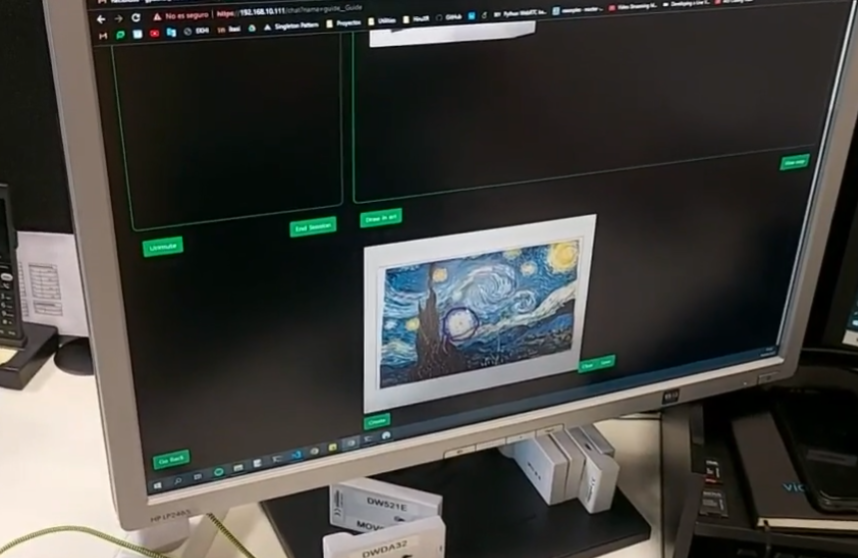
\includegraphics[width=10cm,height=10cm,keepaspectratio]{img/guide drawing.png}
    \caption{Interfaz del guía. Se puede observar la imagen de una obra de arte sobre la que el guía puede dibujar.}
    \label{fig:exmaple_guide drawing}
\end{figure}
\FloatBarrier
Esto puede generar más comprensión por parte del usuario sobre los conceptos explicados, además de poder hacerlo de manera remota sin necesidad de estar allí de manera presencial.


En esta solución se implementa la tecnología \textit{Ultra Wide Band (UWB)} como alternativa a la tecnología \textit{GPS}, debido a que \textit{GPS} no es un sistema de localización fiable dentro de edificios. La localización dentro de edificios (localización \textit{indoor}) se quiere realizar debido a que los usuarios se mueven entre salas. Esto permite hacer \textit{geofencing} y que un usuario pueda ver un mensaje de bienvenida la primera vez que entra a una sala.

Respecto a \textit{UWB}, es similar a la tecnología comunicación muy extendida \textit{Bluetooth Low Energy (BLE)}, pero con mejores prestaciones, para intentar que el sistema sea lo menos propenso a errores y así el cálculo de la localización de los usuarios sea lo más precisa posible. 

En al figura 1.2 aparece representado un sistema típico de interconexión \textit{UWB} para la ubicación de un visitante. En la figura se han utilizado los siguientes términos:
\begin{figure}[t]
    \centering
    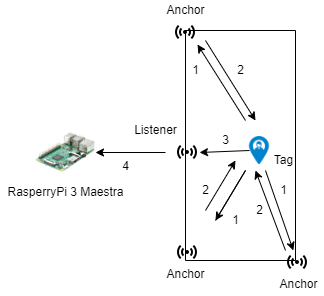
\includegraphics[width=10cm,height=10cm,keepaspectratio]{img/Esquema Conexiones UWB.drawio.png}
    \caption{Disposición de placas \textit{UWB} para la localización \textit{indoor}.}
    \label{fig:exmaple_UWB}
\end{figure}

\begin{itemize}
    \item \textbf{Anchor}: rol que ejerce una placa \textit{UWB} ubicada físicamente en los límites de una sala del museo y que se mantiene estática y pasiva para que otras placas puedan consultar su posición en el proceso de cálculo de la localización.
    \item \textbf{Tag}: rol que ejerce una placa \textit{UWB} transportada por el visitante del museo. Es la encargada de realizar su propia triangulación consultando, en el proceso, la posición de las placas \textit{Anchor}. Una vez calculada su posición se la envía a la placa \textit{Listener} para su gestión.

    \item \textbf{Listener}: rol que ejerce una placa \textit{UWB} encargada de recoger todas las posiciones de las placas Tag y enviárselas a la \textit{Raspberry}.
    \item \textbf{Raspberries Pi 3}: es un ordenador integrado en una placa. Es referenciado como \textit{raspberry}, siendo el intermediario entre la red de placas \textit{UWB} y la \textit{API}, diseñada para la comunicación entre las interfaces de guía y usuario.
\end{itemize}


Una vez se tiene la posición de los usuarios, la idea es representarlo en un mapa a través de una aplicación web o \textit{webapp}, así el guía que esté dando una visita en el museo tendrá más información y contexto del sitio exacto del grupo visitante.

\begin{figure}[t]
    \centering
    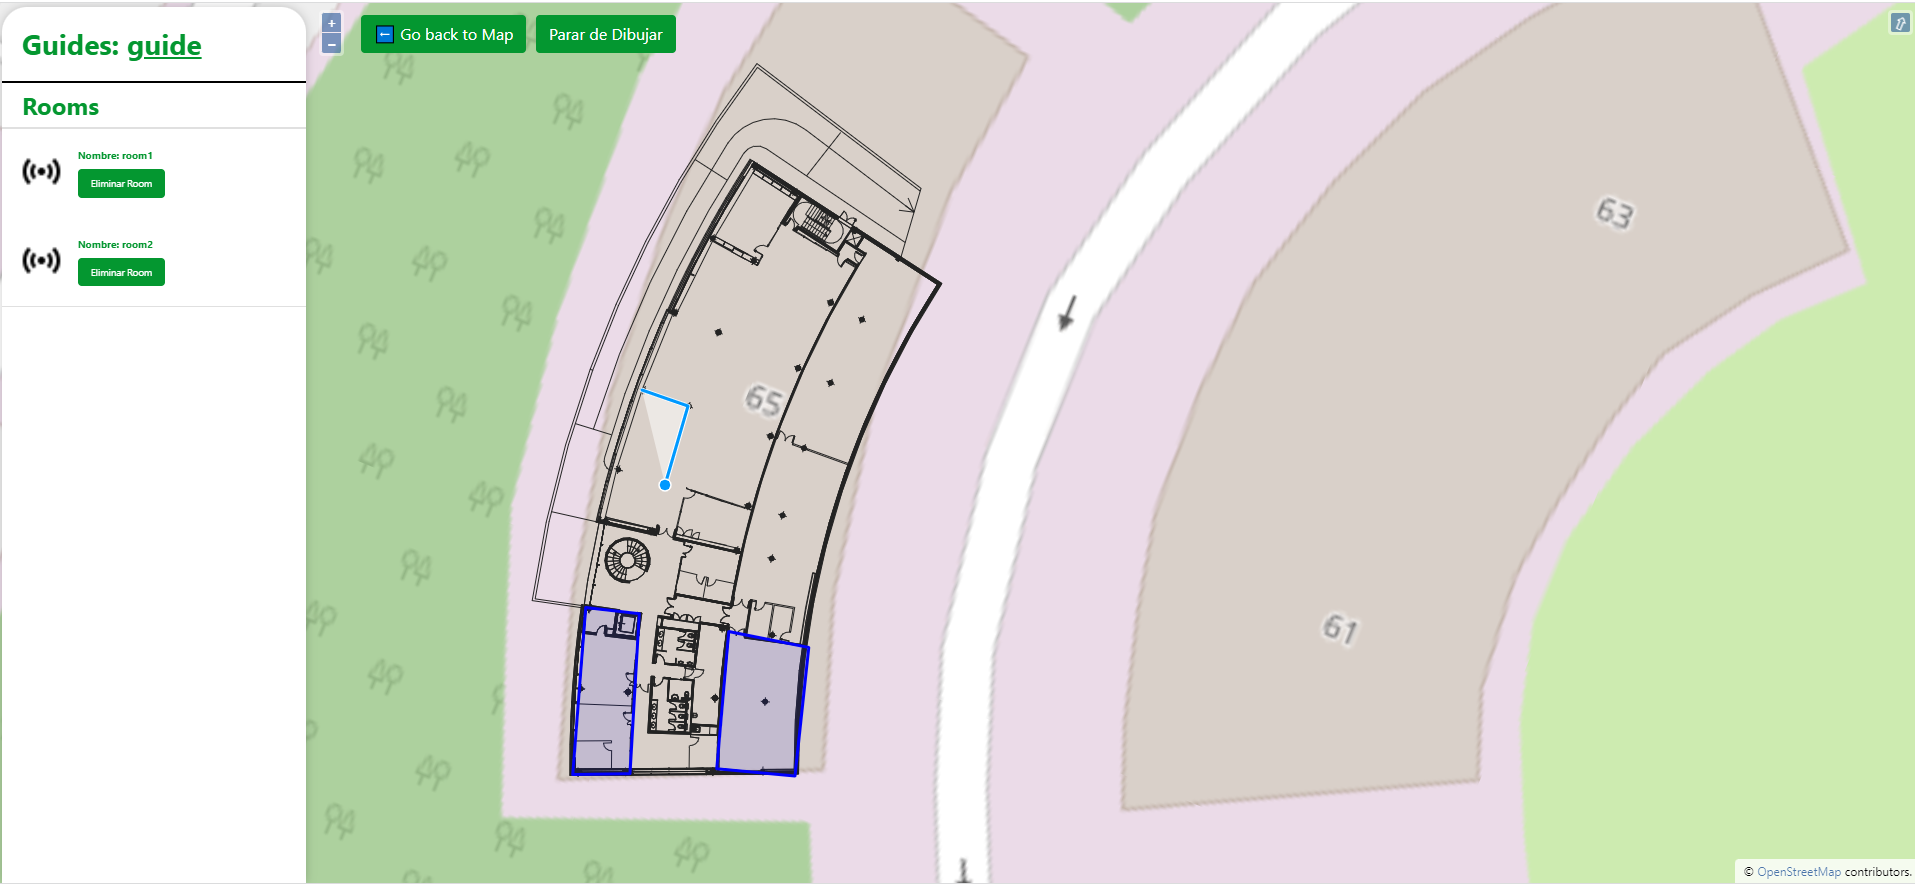
\includegraphics[width=10cm,height=10cm,keepaspectratio]{img/EditRoom.png}
    \caption{Imagen del sistema de dibujado de las salas (en azul). A la izquierda aparece un sidebar con el nombre de todas las salas (rooms) activas.}
    \label{fig:exmaple_room_editing}
\end{figure}

Teniendo la localización en el mapa de los usuarios, el guía podrá crear salas en un mapa dibujándolas, que llamaremos \textit{\textbf{Rooms}}, además contará con un \textit{sidebar} que lista todas las \textit{Rooms} que existen en el sistema, cada una de ellas con un botón que permite su borrado, todo esto mostrado en la figura 1.3.




\section{Estructura de la memoria}
La estructura principal de la memoria será:
\begin{itemize}
  \item \textbf{Introducción}: Descripción general del proyecto. Estructura de la memoria incluida en este apartado junto con los materiales complementarios a la memoria.
  \item \textbf{Objetivos del proyecto}: Explicación de las metas que se han conseguido en el proyecto y cuáles son los objetivos generales tanto a nivel de producto como a nivel de investigación.
  \item \textbf{Conceptos teóricos}: Explicación de los conceptos teóricos necesarios para la realización del proyecto.
  \item \textbf{Técnicas y herramientas}: Descripción de las herramientas y técnicas utilizadas durante la realización de este proyecto.
  \item \textbf{Trabajos relacionados}: Explicación y enumeración de los trabajos necesarios en base a los cuales se han inspirado partes para el desarrollo del proyecto.
  \item \textbf{Conclusiones y líneas de trabajo futuras}: Conclusiones a las que se ha llegado una vez realizado el proyecto y descripción de las diferentes líneas de trabajo futuras.
\end{itemize}
\section{Materiales adjuntos}
Con esta memoria se entrega un dispositivo \textit{USB} que contiene:

\begin{itemize}
  \item La presente memoria en formato \textit{PDF}.
  \item Los anexos en formato \textit{PDF}.
  \item Código fuente de la aplicación Web desarrollada en \textit{React}.
  \item Código fuente de las \textit{Raspberries}. Este código no está en el repositorio por las limitaciones de tamaño de archivos de la plataforma \textit{Github}.
  \item Código fuente de la \textit{API} desarrollada en \textit{Python}.
  \item Vídeo explicativo de los objetivos del proyecto y cuáles han sido las metas conseguidas: \url{https://youtu.be/5EWXAzQejXU}
  \item Repositorio de \textit{Github} con el código parcial de la aplicación: \url{https://github.com/maugvb/tfg-ing-informatica}
\end{itemize}


\capitulo{2}{Objetivos del proyecto}
En esta sección se describirán los distintos objetivos que tienen como meta el desarrollo del proyecto:
\section{Objetivos generales}
\begin{itemize}
  \item Diseñar las interfaces de usuario, la \textit{API}, la interacción entre visitante y guía, y el flujo de los datos.
  \item Desarrollar un asistente para visitar museos implementando \textit{localización indoor} y realidad aumentada.
  \item Desarrollar el asistente en un entorno web con la librería de \textit{javascript} \textit{ReactJS}.
  \item Desarrollar una \textit{API} que dé cohesión a todo el flujo de datos generado entre la generación de datos y la web.
  \item Desarrollar un sistema de posicionamiento \textit{indoor} fiable en base a librerías \textit{Open Source}
  \item Desarrollar una aplicación con las características mencionadas que sea  \textit{Open Source}
  
\end{itemize}
\section{Objetivos en investigación}
\begin{itemize}

  \item Obtener un sistema de precisión mejorado \textit{outdoor/indoor} con una precisión de 0,5 metros en horizontal.
\end{itemize}

\section{Objetivos técnicos}
\begin{itemize}
  \item Desarrollar una aplicación web en \textit{ReactJS} desde cero, que muestre en un mapa los usuarios con una actualización de la posición una vez por segundo (1 Hz).
  \item Crear salas virtuales desde el mapa para poder crear un sistema que indique cuántos usuarios hay en cada una.
  \item Dar a los usuarios experiencia de realidad aumentada implementando un \textit{canvas} con la obra de arte visualizada donde el guía pueda dibujar.
  \item Hacer un sistema de representación local para calcular la localización de los \textit{Tags} y representarlo en un sistema global en formato \textit{EPSG:3857}, que es el estándar de la exportación.
  
\end{itemize}
\section{Objetivos personales}
\begin{itemize}

  \item Obtener conocimientos sobre el posicionamiento en mapas a alta frecuencia.
  \item Obtener conocimientos avanzados sobre \textit{React}.
  \item Obtener conocimientos avanzados sobre la creación de \textit{endpoints}.
  \item Obtener conocimientos sobre \textit{geofencing}.
  \item Obtener conocimientos sobre gestión de \textit{canvas} con la librería \textit{P5}.
\end{itemize}


\capitulo{3}{Conceptos teóricos}
\section{Geoposicionamiento}

El geoposicionamiento es la capacidad de determinar o estimar la posición geográfica de un objeto\cite{GeoPosicionamiento}. Este concepto es fundamental en el proyecto, ya que lo utilizamos para calcular las localizaciones \textit{indoor}.

Para entender en profundidad el proyecto creado, es necesario conocer algunos conceptos que están relacionados con el geoposicionamiento:

\begin{itemize}
    \item \textit{\textbf{GPS}}: Sistema que permite la localización de un objeto sobre la tierra con precisión de hasta centímetros.\cite{wiki:gps}
    \item \textbf{Triangulación}: En el contexto de \textit{GPS} y mediante satélites que mandan señales. Con tres satélites, consiste en averiguar el ángulo de las tres señales respecto al punto de medición. Con esto se consigue la posición relativa respecto a los tres satélites.
    \item \textbf{Localización indoor}: Surge del margen de error de las mediciones \textit{GPS} y se trata de obtener la localización de un usuario dentro de un edificio mediante triangulación. Se replica este sistema a menor escala con distintas placas \textit{UWB} posicionadas de manera que se pueda conseguir la posición relativa de una de ellas respecto a las otras.
\end{itemize}


\section{Interfaz de programación de aplicaciones (API)}
Este concepto sirve para conectar componentes y que se puedan comunicar entre ellos, como por ejemplo una aplicación web y una base de datos.

Se utiliza la arquitectura \textit{Restful}, eso significa que se ha implementado utilizando estos principios \textit{REST}\cite{apiRest}:
\begin{itemize}
    \item \textbf{Sin estado}: La \textit{API} trata a todas las peticiones entrantes por igual, y no guarda información de ninguna de ellas.
    \item \textbf{Operaciones Especificas}: Cada operación es concreta y especifica, no multifuncional.
    \item \textbf{Sintaxis estandarizada}: Cada recurso es accesible únicamente mediante su identificador de recursos uniforme (\textit{URI}), que es el enlace de acceso a un recurso.
    \item \textbf{Cliente-Servidor}: Se utiliza una arquitectura cliente servidor para hacer las peticiones, siendo el servidor el que tiene la lógica de los recursos y los expone al cliente.
En la figura 3.1 se expone la interacción entre la \textit{API}, el cliente y la base de datos
\end{itemize}
\begin{figure}[h]
    \centering
    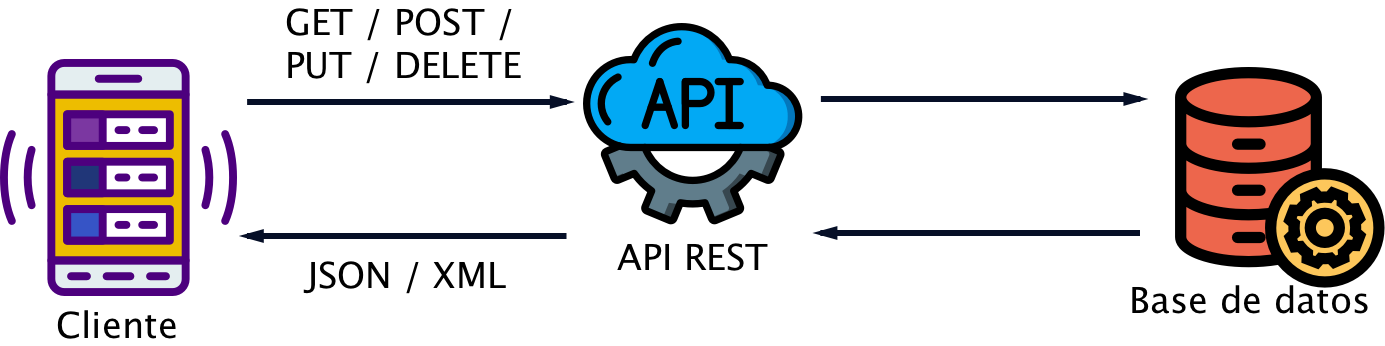
\includegraphics[width=10cm,height=10cm,keepaspectratio]{img/Esquema API.png}
    \caption{Ilustración de conexiones de una \textit{API Rest} \cite{EsquemaAPI}.}
    \label{fig:example_GPS}
\end{figure}
\FloatBarrier
Todos estos conceptos, además, se han desarrollado utilizando el estándar \textit{OpenAPI 3.0} con la ayuda de \textit{Swagger Editor}. 

\textit{OpenAPI} se utiliza para la definición de los componentes de una \textit{API} mediante un archivo de extensión .yaml.
Mediante ese archivo y con la ayuda de la herramienta \textit{Swagger Editor}, se genera un proyecto en \textit{Python} y \textit{Flask} listo para conectar con la base de datos e implementar los métodos de los \textit{endpoints}, que son puntos finales en un canal de comunicación.






\section{Sesiones de usuario}
Para el desarrollo del proyecto, se decidió que los usuarios no iban a tener cuentas de usuario, sino que que se iba a trabajar con sesiones especiales para las pruebas  de la manera más realista.

A un usuario no le interesa tener una cuenta en un museo que seguramente solo vaya a visitar un par de veces, por lo que las sesiones eran la mejor opción. Las sesiones tienen las siguientes características:
\begin{itemize}
    \item Una sesión de usuario en la base de datos, se creará cuando un usuario introduzca en el formulario de Login un alias y el id de su \textit{Tag} asignado.
    \item Cuando un usuario termina la sesión del tour, la fila con su alias no se borra, solo se desenlaza la \textit{Tag}, así más adelante, si otro usuario introduce el mismo alias se reutilizará la sesión.
    \item Si un usuario introduce un alias que está siendo utilizado, no permitirá el enlace con el \textit{Tag}, así que se tendrá que elegir otro alias.
\end{itemize}

\section{Intercambio de Recursos de Origen Cruzado (CORS)}
Este concepto se implementa en las navegadores como medida de seguridad, para las peticiones \textit{HTTP} que se ejecutan.\cite{amazon:CORS}

El uso de \textit{CORS} se utiliza en las cabeceras de las peticiones \textit{HTTP}, para que el servidor las acepte, teniendo que poner distintas cabeceras extra para el correcto funcionamiento de la política, que son:

\begin{itemize}
    \item \textit{\textbf{mode: 'cors'}}: esto implementa el modo \textit{cors} en la petición, no es parte de la cabecera, pero es necesario para indicar el tipo de petición que se quiere utilizar desde el navegador.
    \item \textit{\textbf{Access-Control-Allow-Origin}}: Esta cabecera indica si los recursos pueden ser compartidos con el origen. En el proyecto se utiliza el elemento '*' (wildcard) que indica que no es necesario el uso de credenciales en el servidor.
    \item \textit{\textbf{Access-Control-Allow-Methods}}: Esta cabecera indica los métodos aceptados cuando se accede a un recurso.
    \item \textit{\textbf{Access-Control-Allow-Headers}}: Esta cabecera indica los encabezados que pueden ser utilizados en la petición.
\end{itemize}

Para poder utilizar los endpoints de la \textit{API} se tuvo que encapsular la \textit{API} con una librería llamada \textit{flask-cors}, permitiendo que acepte peticiones con \textit{CORS} que vengan desde los navegadores.
\begin{figure}[b]
    \centering
    \includegraphics[width=10cm,height=10cm,keepaspectratio]{img/GPS-satélites.jpg}
    \caption{Ilustración de la triangulación \textit{GPS} \cite{TringulacionGPS}.}
    \label{fig:example_GPS}
\end{figure}
Esto da una capa extra de seguridad en las peticiones, ya que permite bloquear peticiones potencialmente peligrosas. En el proyecto práctico del TFG realmente no se necesita esa capa extra de seguridad, ya que es un proyecto de investigación, por lo que se ha implementado de la manera más básica posible para simplemente permitir todas las peticiones desde los navegadores.

\section{Localización Indoor}
En esta sección se van a explicar los conceptos correspondientes a la implementación de la localización \textit{indoor}, incluida la representación de las coordenada locales en el mapa.

Para calcular la localización general de un usuario normalmente se utiliza
la tecnologia \textit{GPS}, utilizándose para geolocalizar usuarios en cualquier
punto de la tierra con una precisión de metros, mediante el uso de señales,
triangulando la posición con satélites, como se muestra en la figura 3.2. Sin embargo, en ciertos entornos,
como por ejemplo dentro de un edificio, la señal puede no llegar, haciendo
que no sea posible aplicar la tecnologia \textit{GPS} para la localización \textit{indoor}. 

\begin{figure}[b]
    \centering
    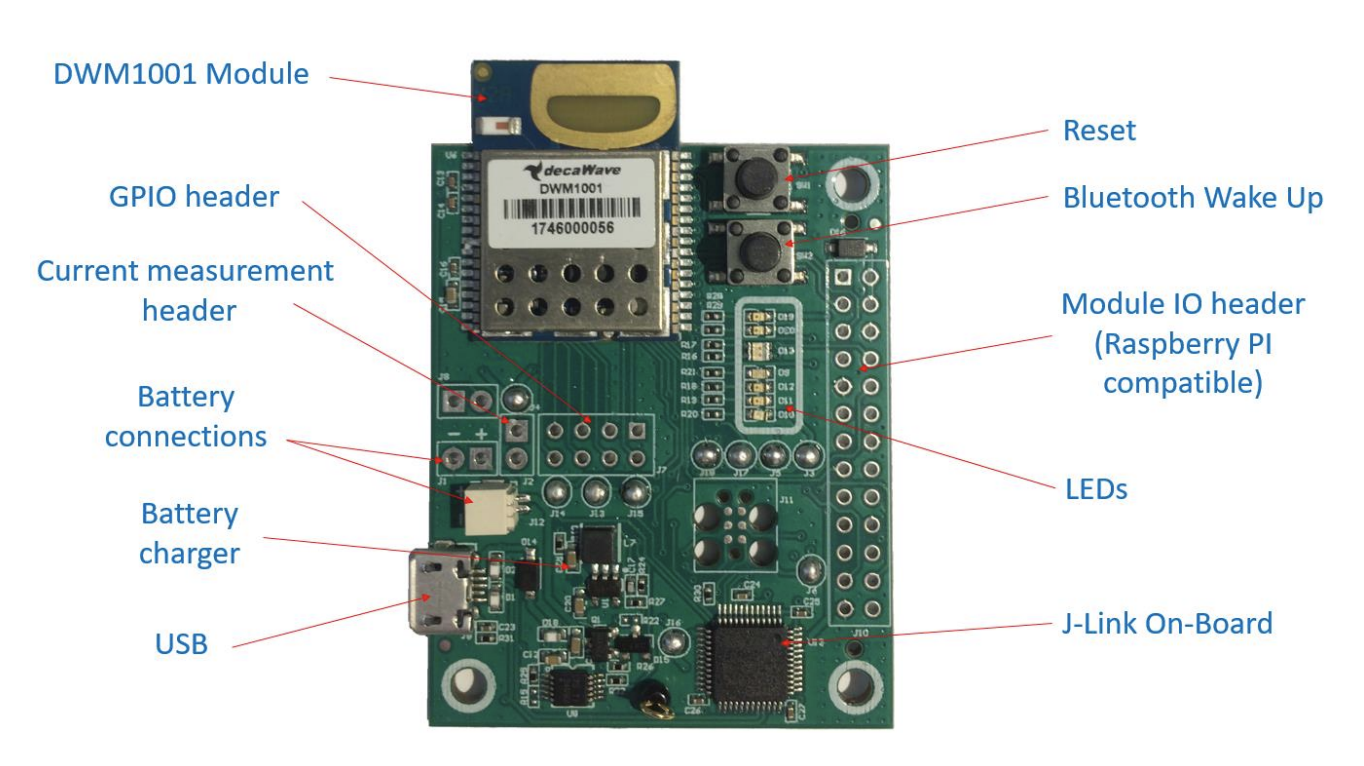
\includegraphics[width=10cm,height=10cm,keepaspectratio]{img/MDEK1001.png}
    \caption{Placa \textit{UWB} MDEK1001 utilizada en este proyecto.}
    \label{fig:example_board}
\end{figure}

De manera general, existen pocas soluciones de localización \textit{indoor} producidas por la investigación a gran escala de estos sistemas, produciendo datos
no tan fiables como los esperados. Haciendo que las soluciones propuestas
hasta el momento, \textit{Wifi} o \textit{Bluetooth Low Energy (BLE)}, no alcancen los
objetivos mínimos necesarios para su implementación en interiores.

\textit{UWB} es el acrónimo de \textit{Ultra Wide Band}, banda ultra ancha, tecnología que utiliza un ancho de banda mayor a 500 MHz\cite{xataka:uwb}. Esta es la tecnología elegida para implementar la geolocalización indoor mediante la triangulación.

El modelo de las placas \textit{UWB} es el \textbf{MDEK1001} usando en el proyecto un total 12 placas, 6 con el rol de \textit{anchors} para consultas pasivas, 2 placas con el rol de \textit{listener}, y 4 con el rol de \textit{tags} como usuarios que triangulan su posición respecto a los demás anchors, trabaja a una frecuencia de 2.4 GHz y tienen una tasa de refresco de 10 Hz.

En la figura 3.3 podemos ver una placa \textit{UWB} modelo \textit{MDEK1001}, con sus distintas partes.


\begin{figure}[t]
    \centering
    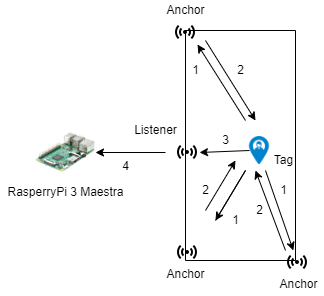
\includegraphics[width=10cm,height=10cm,keepaspectratio]{img/Esquema Conexiones UWB.drawio.png}
    \caption{Esquema de conexiones básico para \textit{localización indoor} en el proyecto.}
    \label{fig:exmaple_indoor_loc}
\end{figure}

Todo este entorno permite trabajar sobre placas \textit{Raspberries Pi 3}, que es un ordenador integrado a modo de placa, como punto de salida con la \textit{API} de cada habitación implementada. La comunicación entre placas \textit{UWB} y \textit{Raspberry} se hace mediante una de las placas, que tiene el rol de \textit{listener}.

Las \textit{Raspberries} funcionan con una arquitectura maestro esclavo y sirven para unificar una red de conexión entre las placas y poder comunicarse con la \textit{API} actualizando la información en el base de datos.

Como las pruebas son con dos entornos pequeños, se han utilizado dos \textit{Raspberries} maestras que se encargan de interactuar con la \textit{API} y las placas \textit{UWB} se mantienen conectadas por la poca distancia que existe entre ellas.

Un ejemplo de triangulación de \textit{UWB} se encuentra en la figura 3.4, donde podemos ver un \textit{Tag} calculado su posición en la representación local respecto a los \textit{anchors} y comunicándoselo al \textit{listener} para que la \textit{Raspberry} mueva esos datos al sistema.





Las \textit{Raspberries} maestras también se encargan de hacer la conversión de la representación local al tipo de datos que pueda utilizar el mapa para representar los elementos.

Esta conversión se hace mediante la traslación del eje de coordenadas X e Y a otro eje Latitud y Longitud. Teniendo las dimensiones de la sala reales en metros, y las coordenadas aproximadas de tres puntos coincidiendo con esquinas de la una sala rectángulo, colocando un \textit{anchor} en cada esquina, convenientemente posicionamos uno de los \textit{anchor} como centro de coordenadas de los ejes X e Y, junto con el ángulo que forman los distintos ejes, mediante trigonometría podemos hacer la traslación de un punto, obteniendo su latitud y longitud reales en el mapa. 

\begin{figure}[t]
    \centering
    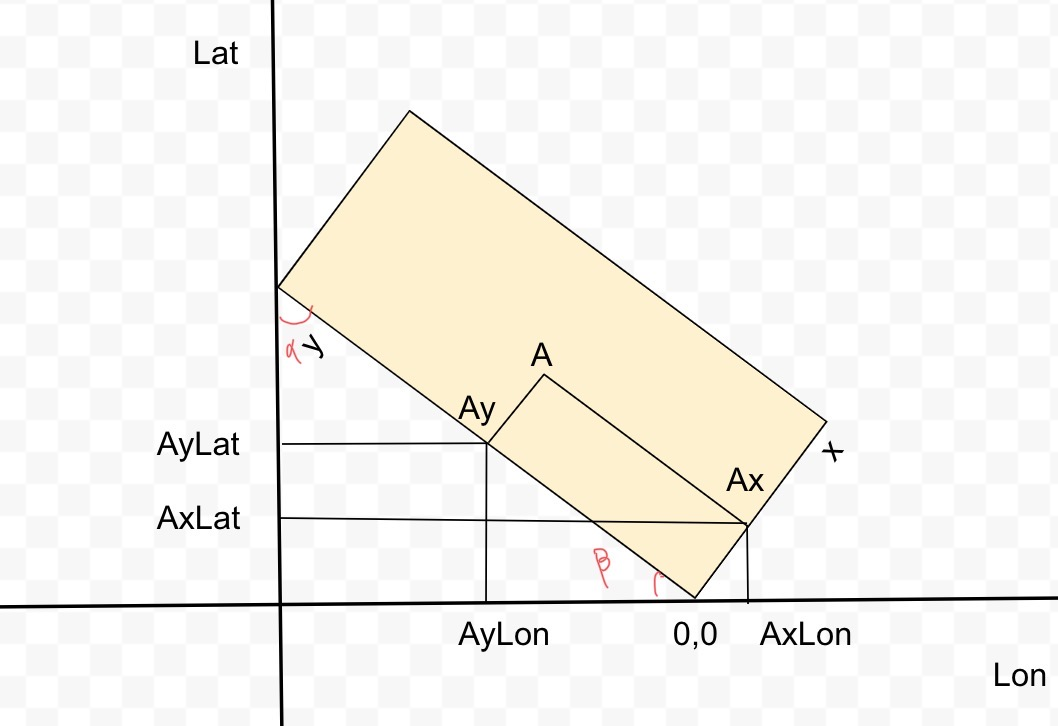
\includegraphics[width=10cm,height=10cm,keepaspectratio]{img/traslation_coorinates.jpg}
    \caption{Conversión de las coordenadas X
e Y a los ejes de Latitud y de Longitud.}
    \label{fig:traslation_coordinates}
\end{figure}


En la figura 3.5 podemos ver como el punto A se proyecta sobre el eje de coordenadas de Latitud y Longitud, teniendo dos puntos sobre estos nuevos ejes del punto principal.


Después, y sabiendo que 1 metro en el mapa equivalen a 120000 metros, que es la escala que utilizamos en el mapa, podemos crear una fórmula general de como hacer la traslación de un punto entre ejes de coordenadas:


\[ diffLat = \frac{Y*sin(ángulo) + X*sin(90 ^{\circ}  + ángulo)}{120000} \]
\[ diffLon = \frac{Y*cos(ángulo) + X*cos(90^{\circ} + ángulo)}{120000} \]

Simplificando queda:



\[ diffLat = \frac{Y*sin(ángulo) + X*cos(ángulo)}{120000} \]
\[ diffLon = \frac{Y*cos(ángulo) + X*sin(ángulo)}{120000} \]

Teniendo en cuenta que el centro de coordenadas de X e Y se tiene como 0,0 y su representación en Latitud y Longitud, el cálculo final de las coordenadas del punto quedaría:

\[ Lat = centerLat + diffLat \]

\[ Lon = centerLon + diffLon  \]

La formula general quedaría:

\[ Lat = centerLat + \frac{Y*sin(ángulo) + X*cos(ángulo)}{120000} \]

\[ Lon = centerLon + \frac{Y*cos(ángulo) + X*sin(ángulo)}{120000}  \]

Una vez calculadas las coordenadas, se implementará una llamada a un \textit{endpoint} para la persisitencia o modificado de las coordenadas en la base de datos.


\section{Geofencing}

El \textit{geofencing} es el proceso de intersecar las coordenadas de uno o más polígonos con las coordenadas de uno o más puntos, dándonos métricas importantes sobre el posicionamiento de los puntos.

Este proceso se puede realizar a tiempo real, y entonces obtenemos cuándo los puntos en movimiento entran a los polígonos estáticos, siendo los polígonos las salas y los puntos los usuarios, creamos el concepto de cuando un usuario entra a una sala y con esto podemos:

\begin{itemize}
    \item Saber en qué sala está un usuario a tiempo real.
    \item Saber cuántos usuarios hay en una sala a tiempo real.
\end{itemize}

En la figura 3.6 podemos ver como un \textit{Tag} se encuentra dentro de una \textit{Room}, por lo que se le puede aplicar \textit{geofencing} para obtener el nombre de la \textit{Room} en la que se encuentra.

\begin{figure}[t]
    \centering
    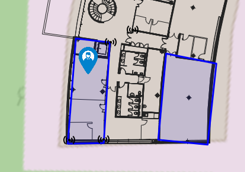
\includegraphics[width=10cm,height=10cm,keepaspectratio]{img/geofencing.png}
    \caption{Sistema de \textit{Geofencing}. Las posición del visitante se interseca con los límites de la \textit{Room} (en azul).}
    \label{fig:traslation_coordinates}
\end{figure}

\capitulo{4}{Técnicas y herramientas}

En esta sección se describirán tanto las herramientas como las metodologías utilizadas, necesarias para la elaboración del proyecto. En la tabla 4.1 aparecen listadas todas las tecnologías.



\tablaSmall{Herramientas y tecnologías utilizadas en cada parte del proyecto.}{l c c c c}{herramientasportipodeuso}{ \multicolumn{1}{l}{Herramientas} & WebApp ReactJS & API & BD & Memoria \\}{ 
REACTJS & X & & &\\
OPENLAYERS & X & & &\\
BOOTSTRAP & X & & &\\
JAVASCRIPT & X & & &\\
REACT-ROUTER-DOM & X & & &\\
ZUSTAND & X & & &\\
P5 & X & & &\\
SASS & X & & &\\
JANUS & X & & &\\
NGINX & X & & &\\
OPENAPI & & X & &\\
PYTHON & & X & &\\
FLASK & & X & &\\
SQLALCHEMY & & X & &\\
MYSQL & & & X &\\
LATEX & & & & X\\
OVERLEAF & & & & X\\
TeXMaker & & & & X\\
DOCKER & & X & X &\\
JSON & X & X & &\\
GIT+GITHUB & X & X & X & X\\
}{t}



\section{Metodologías}
\subsection{Scrum}
Con el uso de esta metodología ágil se consiguió hacer un desarrollo incremental e iterativo de la aplicación, mediante el uso de \textit{sprints} siendo estos los ejes de desarrollo del proyecto.

\section{Patrones de diseño}
\subsection{MODELO VISTA CONTROLADOR (MVC)}
Es un modelo de arquitectura de sistemas utilizado en la parte de la API para la gestión de los datos con la interfaz de usuario.
Se compone de tres partes principales:

\begin{itemize}
    \item \textbf{Modelo}: Es la parte del modelo que se encarga de la lógica de negocio y de la persistencia.
    \item \textbf{Vista}: Esta parte esta formada por los datos enviados al cliente y todas las formas de interacción con ellas.
    \item \textbf{Controlador}: Es la parte que hace de intermediario entre la parte de la Vista y el Modelo generando un flujo de datos y modificándolos para adaptarlo a cada una de las partes si es necesario.
\end{itemize}

En la figura 4.1 podemos ver un esquema que representa la interacción de las distintas partes del modelo \textit{MVC}.
\begin{figure}[t]
    \centering
    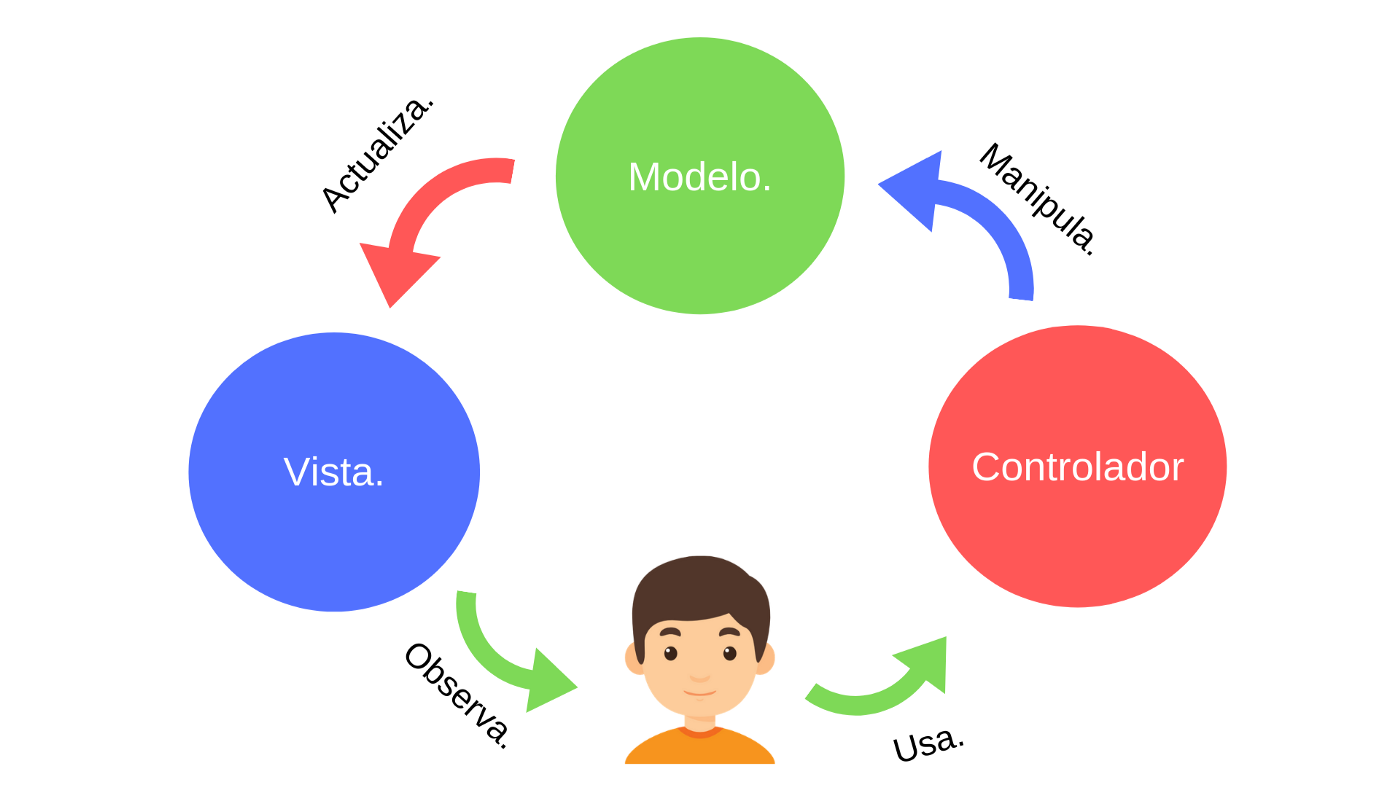
\includegraphics[width=10cm,height=10cm,keepaspectratio]{img/mvc.png}
    \caption{Imagen de \textit{MVC} \cite{mvcImag}.}
    \label{fig:imagen-mvc}
\end{figure}





\subsection{Arquitectura del sistema}

En nuestro caso teniendo en cuenta el modelo \textit{MVC}\cite{mvc}:

\begin{itemize}
\item La parte del \textbf{modelo} estaría en la \textit{API} y se encargaría de crear las bases de datos mediante el \textit{ORM SQLAlchemy}, así como también de generar todas las relaciones entre las tablas. También genera un esquema de cada tabla para poder hacer operaciones con los datos.\item La parte del \textbf{controlador} también estaría en la \textit{API}, teniendo la lógica de interacción, con otras partes del sistema, en cada llamada a los \textit{endpoints}.
\item En \textbf{vista} podríamos considerar la parte de la \textit{webapp} que interactúa mediante los \textit{endpoints} con la \textit{API} para luego mostrar los datos que recibe o hacer operaciones en la base de datos.
\end{itemize}

Podemos ver el esquema general del proyecto en la figura 4.2.

\FloatBarrier
\begin{figure}[h]
    \centering
    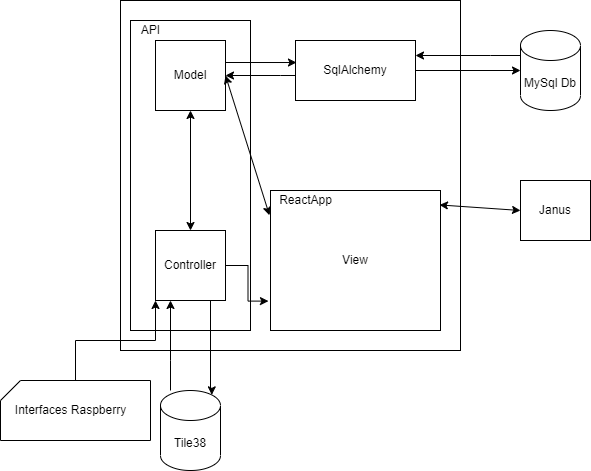
\includegraphics[width=10cm,height=10cm,keepaspectratio]{img/Esquema general del proyecto.drawio (1).png}
    \caption{Esquema del sistema.}
    \label{fig:Esquema-del-sistema}
\end{figure}
\FloatBarrier

\subsection{Maestro-Esclavo}
Esta arquitectura es utilizada principalmente en las \textit{raspberries} cuando queremos escalar el sistema para localizar a usuarios en habitaciones grandes. Tendríamos una \textit{raspberry} maestra que pediría la información a las \textit{raspberries} esclavas, y sería la maestra la que controlaría la información. Al no tener entornos grandes, en este proyecto, solo se han utilizado \textit{raspberries} con rol maestro.

Tendríamos un concepto similar llamado \textit{Follower-Leader}, utilizado en \textit{Tile38}, que es un sistema de \textit{geofencing}, donde tenemos un contenedor con el rol de \textit{Leader} y otro con el rol de \textit{Follower}, así el acceso a los recursos es mucho más rápido.
\section{Control de versiones}
\subsection{GIT}
Se ha utilizado \textit{git} como herramienta de control de versiones, haciendo un registro de versiones mediante \textit{commits} y \textit{branches}, y usando repositorios locales y remotos.
\subsection{GITHUB}
Github es una plataforma de desarrollo colaborativo en la nube, que hace uso de la herramienta \textit{git} alojando código en el repositorio remoto asignado.
\section{Entorno de desarrollo}
\subsection{Visual Studio Code}
\textit{Visual Studio Code} es un editor de código que viene con la herramienta \textit{git} integrada, viene con soporte nativo para lenguajes como \textit{Javascript} y acceso rápido a cualquiera de sus librerías mediante predicción inteligente de escritura, así como soporte para lenguajes de marcas como \textit{HTML} u hojas de estilo como \textit{CSS}.

Este editor cuenta con una selección de \textit{plugins} de la comunidad que le hacen compatible para escribir código con muchísimos lenguajes del mercado.
\subsection{DBeaver}
Se ha utilizado \textit{DBeaver} como cliente de \textit{SQL}, esta herramienta ha sido muy útil durante el desarrollo del proyecto permitiendo consultar, escribir modificar o borrar datos y/o estructuras de las tablas en cualquier momento con una interfaz gráfica.
\section{Documentación}
\subsection{TeXMaker}
Es un procesador de texto multiplataforma que permite crear documentos en \LaTeX y exportarlo a diferentes formatos.
\subsection{Overleaf}
Procesador de texto colaborativo, online, que permite la escritura de documentos en \LaTeX y su exportación en diferentes formatos.
\section{Herramientas para el desarrollo}
\subsection{Docker}
Herramienta que permite la automatización del despliegue de distintos tipos de aplicaciones, funciona con contenedores que se basan en imágenes y proporciona una capa de abstracción para la virtualización de servicios.
\subsection{NGINX}
Herramienta que permite el despliegue de un servicio web, creando un servidor web que atiende peticiones.
En este proyecto esta herramienta se ha utilizado como \textit{reverse proxy} para atender peticiones por \textit{HTTPS }y redirigirlas a un dirección y puerto de la \textit{API} por \textit{HTTP} y desplegándola con \textit{docker}.
\subsection{MYSQL}
Sistema de gestión de bases de datos creada por \textit{Oracle}, el cual crea un servidor para dar servicio y que los clientes se conecten para poder interactuar con las tablas o con alguna base de datos.
\subsection{Javascript}
Lenguaje de programación orientado a cliente y se interpreta de manera nativa en los buscadores modernos.
\subsection{SaSS}
Tipo de lenguaje de hoja de estilos que añade más posibilidades que las hojas de estilos convencionales a la hora de programar, haciendo que las hojas de estilo de \textit{SaSS} sean fácil la tarea de mantener con grandes secciones de código.


\section{Librerías}
\subsection{ReactJS}
\textit{ReactJS} es una biblioteca de \textit{Javascript} creada por \textit{Facebook}, con la finalidad de crear aplicaciones de una sola página dinámicas.

Se basa en el concepto de componentes y estado. Donde un componente es una pieza de código, con similitudes a una clase en \textit{Java}, donde se definen e implementan los métodos, además tiene un método \textit{render}, de obligatoria llamada, que devuelve código \textit{jsx} muy similar a \textit{HTML}.\cite{React}

Un componente puede ser llamado por otro en la función \textit{render} como etiqueta, todo lo que se le pase como atributos será accesible como propiedades dentro del componente.

El estado del componente son todas aquellas variables que van a ser definidas para el propósito del componente, son constantes y se modifican a través de funciones implícitas de \textit{React}.

Existen dos tipos de componentes:
\begin{itemize}
    \item \textit{\textbf{Statefull Component}}: es un componente con estado, su responsabilidad es cambiar o mantener el estado, y pasarlo como atributos si es necesario.
    \item \textit{\textbf{Stateless Component}}: es un componente sin estado, solo muestra información estática o información pasada como propiedades.
\end{itemize}

Todo esto se ha modernizado en las últimas versiones de \textit{React} con la implementación de \textit{hooks}, que son métodos implícitos que utilizan el concepto de componentes de manera interna, simplificando el desarrollo tan rígido de los componentes.

Para la gestión de las páginas en \textit{React}, se utiliza una librería llamada \textit{react-router-dom}, que en el componente raíz, permite gestionar la ruta de la página y el componente a procesar por el buscador. El uso de esta librería hace que cambiar de página sea una simple llamada a la \textit{api} de la librería.

Además en algunas partes de la aplicación se requirió utilizar un estado compartido entre componentes independientes. Para esto se utilizó \textit{Zustand}, que es una librería que permite este funcionamiento. Este comportamiento no es recomendable en \textit{React}, ya que puede haber fugas de memoria, así que minimizamos el estado compartido lo máximo posible.
\subsection{React-router-dom}
Librería \textit{javascript open source} para controlar la navegación entre páginas de manera sencilla. Se basa en definir en el componente raíz unas rutas a las cuales podemos acceder con llamadas a la \textit{api} de la librería para representar gráficamente, en el buscador un componente a modo de página.
\subsection{Zustand}
Librería \textit{javascript open source} para poder tener un estado global accesible desde componentes independientes en \textit{React}.
\subsection{P5}
Librería \textit{javascript open source} para poder representar gráficamente objetos. Permite la posibilidad de desarrollar un sistema de dibujado, sobre un área concreta. En este trabajo se emplea para dibujar sobre las imágenes de las obras de arte que el visitante del museo está visualizando en su dispositivo. \cite{P5} 

Se basa en crear un \textit{canvas} de fondo, solo para la representación gráfica de una imagen, y posteriormente crear otro \textit{canvas} transparente encima, donde habilitaremos la opción de dibujar, pudiendo así dibujar encima de la imagen.

Esto se activará cuando la realidad aumentada detecte una obra de arte, y todo lo dibujado se guardará en la base de datos para su persistencia.

\subsection{OpenLayers}
Es una librería que se utiliza para la implementación de mapas. Su característica principal es que utiliza capas como unidad básica para la representación. Para que el objeto mapa identifique las capas, se utilizan los vectores que puede agrupar una o más \textit{features} como una capa que se visualiza en el mapa.

Las \textit{features} son objetos con la información mínima para la representación en el mapa. A estos objetos se les puede aplicar un estilo permitiendo cambiar, por ejemplo, la imagen a mostrar en el mapa.

En este proyecto para la representación del mapa se utiliza una capa tipo \textit{Tile}, y una capa \textit{Vector} agrupando todo el \textit{GeoJson} de la importación del edificio en la ubicación que queremos, siendo estas dos las capas principales.


Las capas de los \textit{tags} y \textit{anchors} son capas \textit{Vector} con un \textit{source} de un objeto \textit{Feature}. Sin embargo las \textit{Rooms} son capas \textit{Vector }con una \textit{source} de tipo \textit{Polygon}. Esto porque los \textit{tags} y \textit{anchors} se basan solo en una coordenada y las \textit{rooms} en varias. Todas estas coordenadas utilizadas se incluyen en una variable en formato \textit{geoJSON}, que es una porción de código con sintaxis \textit{JSON} pero que se utiliza para la representación de un objeto en el mapa.
\subsection{Bootstrap}
Librería \textit{open source} para la creación de interfaces web mediante el uso de hojas de cascada.
\subsection{Janus}
Librería basada en \textit{WebRTC} para el \textit{stream} de diferentes tipos de datos. En este proyecto se ha utilizado un \textit{docker} como servidor con un \textit{docker} y un cliente web \textit{javascript}.
\subsection{Flask}
\textit{Framework} de \textit{Python} que permite la creación de aplicaciones web. Esta herramienta se ha utilizado para la creación de \textit{endpoints} de la \textit{API} a modo de servidor con \textit{docker}.
\subsection{SQLAlchemy}
Herramienta que permite utilizar los datos de la base de datos como objetos en \textit{Python} permitiendo el llamado \textit{ORM (Object Relational Map)}.

\section{Estándares}
\subsection{JSON}
Estándar para el intercambio de datos entre servicios.
\subsection{GEOJSON}
Es un estándar de de representación geográfica de elementos sencillos. Está basada en formato \textit{JSON}, por lo que se puede enviar y persistir en formato de \textit{string} de manera simple. \cite{GeoJson}
\subsection{OPENAPI}
Estándar para la definición de \textit{API's}.


\capitulo{5}{Aspectos relevantes del desarrollo del proyecto}

El desarrollo de este trabajo se ha estructurado en varias partes.
Por un lado, el desarrollo de la aplicación web que tiene que interactuar con el visitante del museo y el guía remoto. Por otro lado, también se ha desarrollado la API encargada de interconectar ambos elementos.
Además, con el fin de mejorar tanto la organización de las visitas guiadas como la experiencia del visitante, también se ha implementado un sistema de geolocalización \textit{indoor} basado en tecnología \textit{UWB}.
Por último, en este trabajo también se ha participado en parte del desarrollo del dibujado sobre obras de arte por parte del guía para su representación gráfica en el usuario, siendo este uno de los puntos claves para la realidad aumentada del proyecto.
\begin{comment}

Este apartado pretende recoger los aspectos más interesantes del desarrollo del proyecto, comentados por los autores del mismo.
Debe incluir desde la exposición del ciclo de vida utilizado, hasta los detalles de mayor relevancia de las fases de análisis, diseño e implementación.
Se busca que no sea una mera operación de copiar y pegar diagramas y extractos del código fuente, sino que realmente se justifiquen los caminos de solución que se han tomado, especialmente aquellos que no sean triviales.
Puede ser el lugar más adecuado para documentar los aspectos más interesantes del diseño y de la implementación, con un mayor hincapié en aspectos tales como el tipo de arquitectura elegido, los índices de las tablas de la base de datos, normalización y desnormalización, distribución en ficheros3, reglas de negocio dentro de las bases de datos (EDVHV GH GDWRV DFWLYDV), aspectos de desarrollo relacionados con el WWW...
Este apartado, debe convertirse en el resumen de la experiencia práctica del proyecto, y por sí mismo justifica que la memoria se convierta en un documento útil, fuente de referencia para los autores, los tutores y futuros alumnos.
- Base de datos
- Uso de React
- Uso de Enpoints
- Uso de Raspberrys
- Uso de OpenAPI
- Uso de Arquitectura pasiva para la triangulación
\end{comment}

\section{Desarrollo de la aplicación web}
Para el desarrollo de la aplicación web había que tener en cuenta la presencia de dos tipos de usuario, visitante del museo y guía remoto. Por el lado del visitante tendríamos el inicio de sesión en el sistema para recibir el vídeo y el audio del guía, y por el lado del guía tendríamos que insertar la geolocalización de cada visitante en su sala y el \textit{canvas} para poder dibujar sobre las imágenes recibidas desde los visitantes.

Durante el desarrollo de la aplicación surgieron diferentes momentos en los que se tuvieron que tomar distintas decisiones sobre cómo desarrollar el software o qué tecnología utilizar, sobre todo en la fase de investigación.

Dado que la interfaz del guía debe incluir la localización de los visitantes, en las primeras fases del proyecto surgieron distintas soluciones para decidir qué librería de mapas se podría utilizar:

\begin{itemize}
    \item \textbf{Carto}. Es un software de bases de datos de alto rendimiento para integración de mapas, compatible con implementaciones de distintos tipos de servicios de localización a tiempo real. La desventaja es que el software de su API web proporcionado es de pago y no es código abierto en su totalidad.
    \item \textbf{Leaflet} - Usando mapa de \textit{OpenStreetMap}. Librería para el desarrollo de mapas en diferentes entornos. En este proyecto en particular se tuvo en cuenta su librería de \textit{javascript}, es de código abierto, pero no cuenta con muchas funcionalidades para la interacción con los usuarios.
    \item \textbf{OpenLayers}. Es otra librería para el desarrollo de mapas, normalmente en entornos web. Se utilizó su versión de \textit{javascript}, debido a que su código era abierto y es una de las librería de mapas más completas que existen a día de hoy para la interacción con los usuarios. 
    \item \textbf{Google Indoor Location}. Solución software de Google para mostrar usuarios en interiores. Se descartó esta solución debido a que solo permitía el uso de la API de mapas de Google.
    \item \textbf{MapWize}. Solución para mostrar usuarios en entornos \textit{indoor}. Se descartó por ser de pago y ya tener un prototipo con herramientas \textit{open source}.
\end{itemize}

Se tenía pensado desde un principio que \textit{React} iba a ser la librería a utilizar,
debido a que se contaba con experiencia previa desarrollando con este \textit{framework} y 
así agilizaría todo a la hora de crear código para el entorno web.

Se creó un proyecto por separado de \textit{OpenLayers} en \textit{Javascript Vainilla} a modo de prueba de concepto para poder implementar una versión básica del mapa, para poder entender los conceptos de cómo funcionan los mapas en la librería y cómo implementarlos con \textit{Javascript}.

En la figura 5.1 se puede ver una implementación de un mapa con \textit{OpenLayers} donde se muestra un \textit{Tag} en azul, un \textit{Anchor} con un cuadrado rojo, que indica que ha sido movido y no guardado en la base de datos, y dos \textit{Rooms}.
\begin{figure}[t]
    \centering
    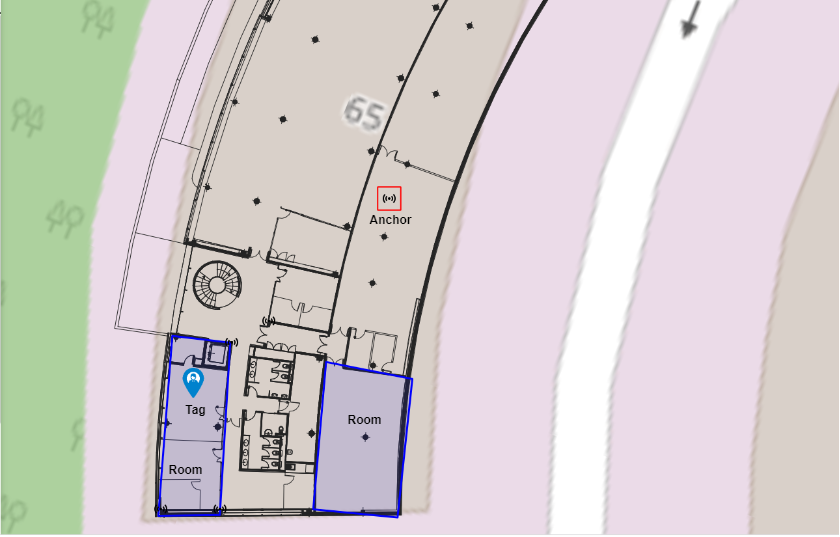
\includegraphics[width=10cm,height=10cm,keepaspectratio]{img/OpenLayers.png}
    \caption{Mapa con OpenLayers con un Tag, dos Rooms y un Anchor con bordeado rojo.}
    \label{fig:Example OpenLayers}
\end{figure}

Llegó un reto importante que era exportar como una capa los planos del edificio donde se iban a realizar las pruebas de despliegue, que en este caso iban a ser las oficinas de Vicomtech. Para realizar este procedimiento se utilizó un software especifico de mapas llamado \textit{QGIS}, el cual fue bastante complejo de entender debido a que está orientado a arquitectos y topógrafos profesionales, por lo que utilizaba terminología desconocida hasta el momento.

Para la exportación de los planos, se importó de un proyecto Autocad como una capa y otra capa sería el mapa en sí. Una vez se tuvieron las capas juntas se procedió a colocar la capa de la estructura en la posición dónde se necesitara, cambiando el centro de coordenadas y el formato de exportación del mapa a \textit{EPSG:3857}, compatible con la librería. 

En la figura 5.2 se puede ver la base del edificio superpuesto como capa en el mapa.

\begin{figure}[t]
    \centering
    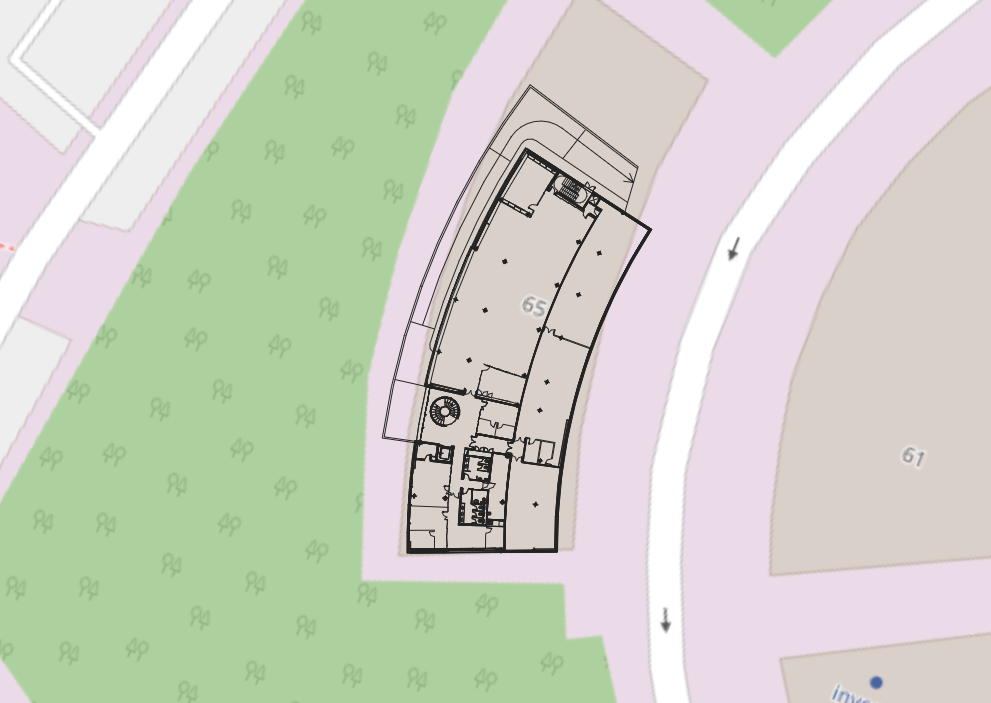
\includegraphics[width=10cm,height=10cm,keepaspectratio]{img/Base Edificio.png}
    \caption{Base de edificio en mapa con \textit{OpenLayers}.}
    \label{fig:Example OpenLayers}
\end{figure}
Una vez en este punto se utilizó un \textit{plugin} del propio \textit{software} que exportaba el proyecto \textit{QGIS} en una web estática con los siguientes elementos:

\begin{itemize}
    \item \textit{HTML} con las etiquetas necesarias para la inicialización del mapa.
    \item \textit{CSS} con los estilos básicos para la visualización del mapa.
    \item \textit{Javascript} con la importación de \textit{OpenLayers} y todo el uso de las funciones de la librería para la creación de capas e inicialización del mapa en la etiqueta asignada.
\end{itemize}

La creación de la capa de los planos se hacía mediante la exportación de la capa a un \textit{JSON} en formato \textit{EPSG:3857} Mismo formato que el mapa, esto se desarrolló en el proyecto estático donde ya existía una implementación de la librería con algunas interacciones referentes al mapa programadas previamente.

Tras esto tocó adaptar la librería \textit{OpenLayers} a \textit{ReactJs}, ya que no existía ninguna que adaptara \textit{OpenLayers} \textit{(Javascript Vainilla)} a componentes \textit{React}. Esto llevó un tiempo considerable, ya que tocó reescribir las funciones de inicializado de mapas en un componente \textit{React}, combinando la sintaxis de los componentes con la sintaxis de \textit{Javascript} puro.

Una vez existía interacción entre la aplicación \textit{React} y la \textit{API} tocó implementar distintas funcionalidades que mejoraran la experiencia de usuario cómo:

\begin{itemize}
    \item Mostrar a los \textit{Anchors} en el mapa, poderlos mover, y que se pueda persistir la nueva posición. También se añadió un bordeado rojo para aquellos \textit{Anchors} que se muevan y no se guarden.
    \item Mostrar a los \textit{Tags} ligados a usuarios en el mapa, en base a la posición de las coordenadas de la base de datos.
    \item Mostrar \textit{Rooms} existentes en la base de datos como un polígono. También se añadió una página para poder eliminar y añadir \textit{Rooms} dibujando en el mapa.
\end{itemize}

Para mejorar la experiencia de usuario se implementaron unas restricciones en el \textit{login} de los usuarios normales, para comprobar que el usuario no estaba ligado ya a esa sesión o que estaba siendo usado.

Posteriormente a esto, y como último paso, se implementó una función que comprobara el estado de los \textit{tags} con usuarios en la base de datos, y que de manera dinámica identificara qué capas hacía falta borrar, actualizar o añadir en base a la información recibida a 1 Hz, coincidiendo con el la frecuencia de actualización de los Raspberries en la base de datos.

Después se implementó un sistema de dibujado mediante sobreposición de \textit{canvas}, colocando un \textit{canvas} con la obra de arte en el fondo y el \textit{canvas} de dibujado encima, así conseguimos que se pueda dibujar en la obra de arte. Ejemplo de esto se muestra en la figura 5.3.

\FloatBarrier
\begin{figure}[h]
    \centering
    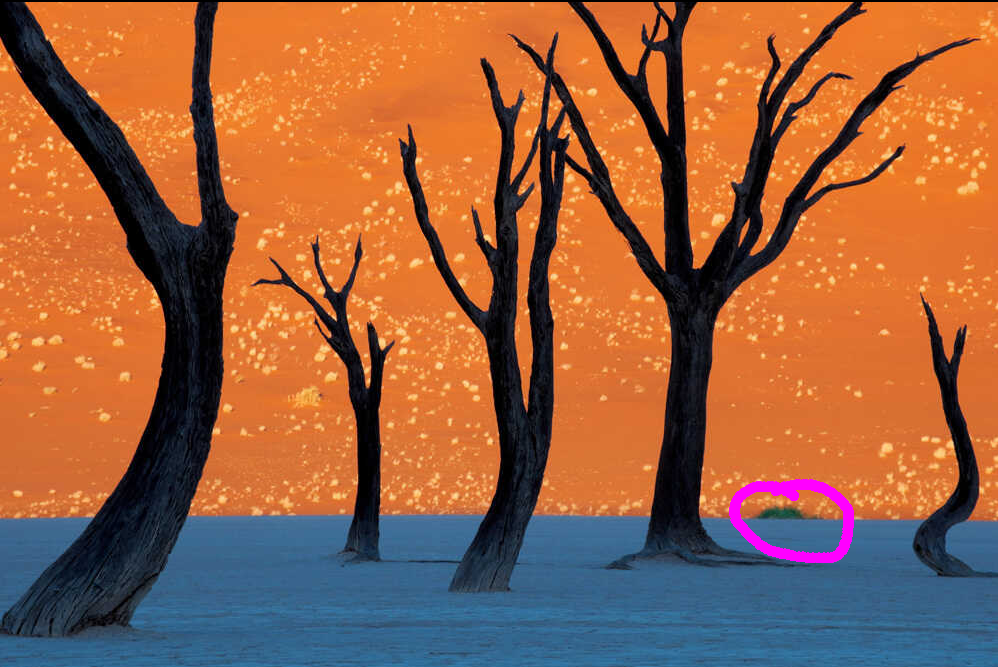
\includegraphics[width=10cm,height=10cm,keepaspectratio]{img/P5Example.png}
    \caption{Dibujado en dos capas con librería \textit{P5}.}
    \label{fig:Example-P5}
\end{figure}
\FloatBarrier
\section{Desarrollo de la API}
Para el desarrollo de la \textit{API} se ha utilizado el estándar \textit{OpenAPI}. Esto permitió utilizar la herramienta \textit{Swagger Editor} (figura 5.4) para escribir las especificaciones necesarias en base a un documento con extensión \textit{yaml}. Este incluye tanto el diseño de los casos de uso como el diseño de los \textit{endpoints} que se iban a utilizar. Esta herramienta permitió poder auto generar una versión de la \textit{API} con \textit{Python} y \textit{Flask}, todo implementado con \textit{docker}.

\begin{figure}[t]
    \centering
    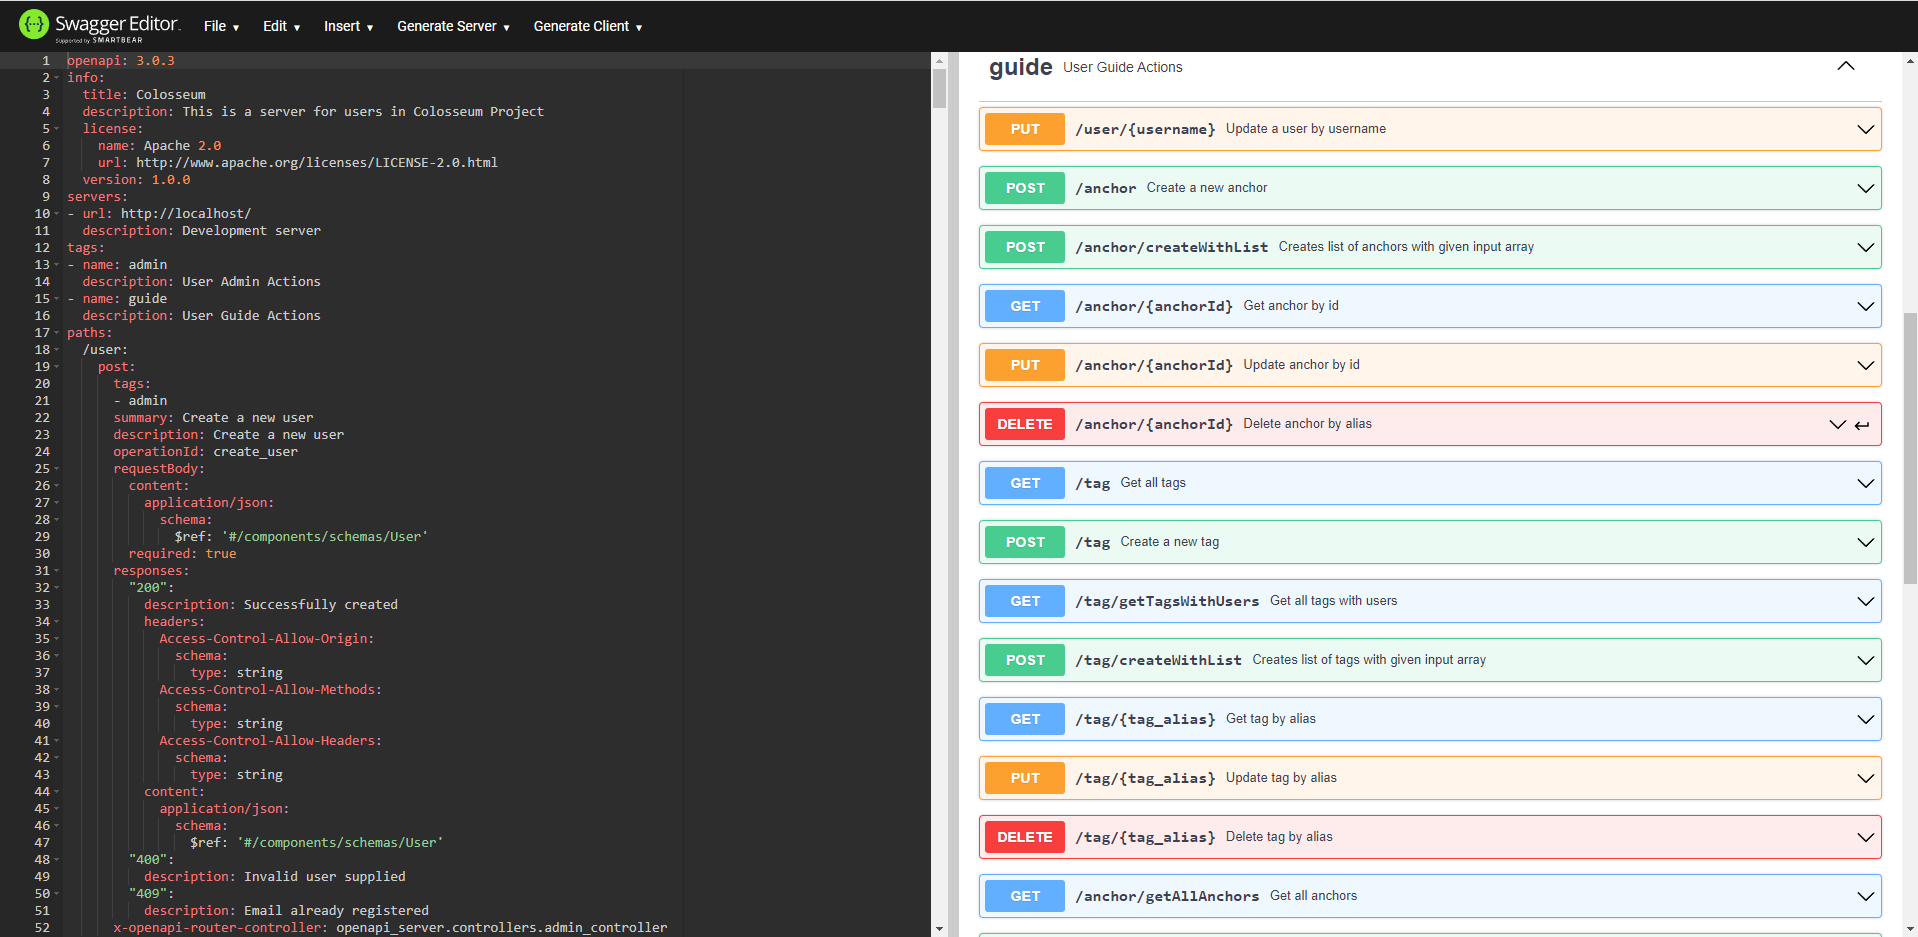
\includegraphics[width=10cm,height=10cm,keepaspectratio]{img/SwaggerEditor.png}
    \caption{Herramienta web \textit{Swagger Editor} con las especificaciones de la \textit{API}.}
    \label{fig:Swagger Editor}
\end{figure}
A esta primera versión auto generada se le tuvo que añadir la librería \textit{Connexion}, para poder generar acceso a los \textit{endpoints} por HTTP en base a la especificación del documento \textit{yaml}.

Para la conexión con la base de datos se añadió:
\begin{itemize}
    \item \textit{\textbf{SqlAlchemy}}, para la gestión de la base de datos a modo de objetos en\textit{Python}.
    \item \textit{\textbf{Marshmellow}}, librería que funciona a modo de \textit{wrapper} necesaria para el funcionamiento de \textit{SqlAlchemy}.
\end{itemize}

Una vez llegados a este punto se tuvo en cuenta la posibilidad de implementar bases de datos óptimas para operaciones con mapas como:
\begin{itemize}
    \item \textit{\textbf{CartoDB}}, una implementación de una base de datos de alto rendimiento basada en \textit{Redis} e implementada por la empresa \textit{Carto}.
    \item \textit{\textbf{MySQL}} como instancia con \textit{Docker}. Al necesitar crear distintas tablas personalizadas para la aplicación, esta opción fue la más flexible para realizar el desarrollo, ya que todo el proyecto se encapsuló en \textit{Docker} para poder automatizar el despliegue y eso lo hizo más compatible con el \textit{ORM SQLAlchemy}.
\end{itemize}

Finalmente se acabó utilizando una instancia \textit{MySQL} en \textit{Docker}  previamente configurada, lo que permitió hacer una conexión rápida a través del \textit{ORM} en la \textit{API}.

Una vez tuvimos todo configurado y conectado, se pasó a realizar la lógica en la parte de los controladores, manejando todas las instrucciones que interactúan con la base de datos que van a ser recibidos por peticiones \textit{HTTP}, e incluso manejando la lógica independiente para añadir, modificar, consultar, eliminar o intersectar objetos en las funcionalidades de \textit{geofencing} \textit{Tile38} utilizando su librería cliente \textit{pyle38}.

\section{Despliegue}
Para el despliegue de la aplicación  web se utilizó una instancia de \textit{Docker} de \textit{Nginx} previamente configurada. Esto permitió un despliegue de la aplicación web a producción de manera que fuese lo más rápido y óptimo posible. Para esto, en vez de utilizar el servidor \textit{HTTP} que compila el código escrito en \textit{react} llamado \textit{react-scripts}, utilizamos \textit{Vite}, que era similar en funcionalidades pero mucho mas rápido, reduciendo así los tiempos para el despliegue y compilación de la aplicación.


\section{Sistema de geolocalización \textit{indoor}}

En las primeras etapas del proyecto se tuvo que analizar qué tipo de tecnología que se iba a utilizar para la geolocalización teniendo en cuenta parámetros como
la latencia de la comunicación, la frecuencia aproximada a la que trabajan los dispositivos de las distintas tecnologías o la resistencia ante interferencias que tengan los dispositivos seleccionados para la fiabilidad de los datos.

Finalmente se consideró utilizar placas \textit{Ultra Wide Band} debido a que en un futuro no muy lejano, gran parte de los teléfonos inteligentes tendrán un \textit{chip} UWB incluido, lo que hace que sea una tecnología muy prometedora.

Para toda la implementación de sistema de geolocalización se utilizaron placas \textit{MDEK1001 UWB} a las que se le cambió el \textit{firmware}, debido a que necesitábamos tener los \textit{anchors} como dispositivos pasivos que reciben y responden comunicaciones, los \textit{tags} para comenzar las comunicaciones, y otras placas actuando como \textit{listener} para comunicarnos con la \textit{raspberry}. Estos roles permitieron crear una arquitectura de placas pasivas-activas, donde la placa o \textit{tag} activa se comunica con los dispositivos pasivos para triangular su posición en el sistema de representación local.

Una vez que se conoce su representación local de las \textit{tag}, se comunican con la placa que hace de \textit{listener}. Esta placa hace de intermediaria entre la \textit{raspberry} y las \textit{tags}, y su función consiste en recibir las posiciones de las placas \textit{tag} y enviárselas a la \textit{raspberry}.

Tras la recepción de las posiciones en la \textit{raspberry}, su función ahora es filtrar \textit{tags} para no obtener duplicados, y hacer la traslación de coordenadas de la representación local a la representación compatible para su representación en el mapa.


En las \textit{Raspberries} al principio se implementó un \textit{firmware} de \textit{FIND3}, que hace de servidor unificando los datos de las conexiones de los \textit{tags UWB}. Crea un servicio web en el que se pueden ver estadísticas e incluso puede utilizar modelos entrenados para hacer \textit{geofencing}. Además \textit{FIND3} cuenta con una \textit{api} para que puedas interactuar con el servicio. Finalmente se implementó un software desde cero debido a que \textit{FIND3} no tenía la precisión necesaria que requería el proyecto.


Las placas \textit{MDEK1001} elegidas pueden ser consultadas mediante una \textit{app} para \textit{Android} vía \textit{Bluetooth Low Energy (BLE)}, permitiendo así modificar su configuración  y ver su ubicación local en una interfaz gráfica.

En la figura 5.5 se puede ver una imagen de un sistema de placas \textit{UWB} donde un \textit{Tag}, representado con un círculo morado, triangula de manera activa su posición en la representación local, en función de los \textit{Anchors}, representados como triángulos rojos, que actúan de manera pasiva.

\begin{figure}[t]
    \centering
    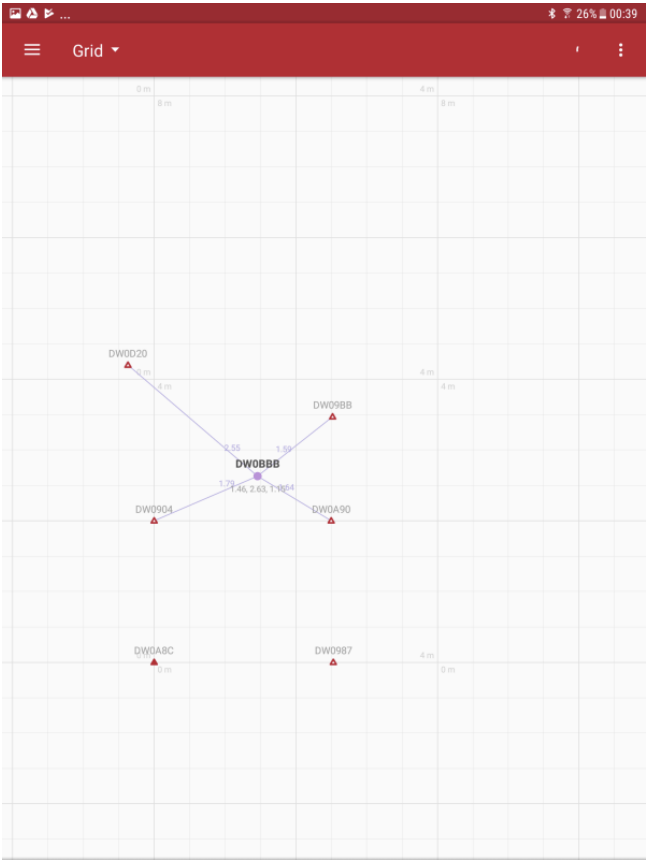
\includegraphics[width=10cm,height=10cm,keepaspectratio]{img/LocationTags.png}
    \caption{Aplicación del fabricante donde se muestra la ubicación local de un \textit{tag}.}
    \label{fig:app-local-representation}
\end{figure}



\section{Pruebas}
Las pruebas de la aplicación se han basado en el rendimiento de las placas en diferentes entornos realistas y su representación en el mapa en tiempo real. 

Los casos probados fueron:
\begin{itemize}
    \item Una sala con 3 \textit{Anchors}, un 1 \textit{Tag}, 1 \textit{Listener} y 1 \textit{Raspberry} para su triangulación y diferentes cuadros colgados en la habitación para probar la realidad aumentada creada para las visitas del guía.
    \item Dos sala con 3 \textit{Anchors} cada una, un 1 \textit{Tag}, 2 \textit{Listener} y 2 \textit{Raspberry} para su triangulación y diferentes cuadros colgados en la habitación para probar la realidad aumentada creada para las visitas del guía.
    \item Una sala con 3 \textit{Anchors}, un 3 \textit{Tags}, 1 \textit{Listener} y 1 \textit{Raspberry} para su triangulación y diferentes cuadros colgados en la habitación para probar la realidad aumentada creada para las visitas del guía.
    \item Dos sala con 3 \textit{Anchors} cada una, un 4 \textit{Tag}, 2 \textit{Listener} y 2 \textit{Raspberry} para su triangulación y diferentes cuadros colgados en la habitación para probar la realidad aumentada creada para las visitas del guía.
\end{itemize}

En la figura 5.6 se muestra el tercer caso de prueba donde existen 3 \textit{Tags}, 3 \textit{Anchors} y 1 \textit{Listener} en una sala física, con el esquema de flujo de de datos. Siendo la prueba más compleja de una sala.

\begin{figure}[t]
    \centering
    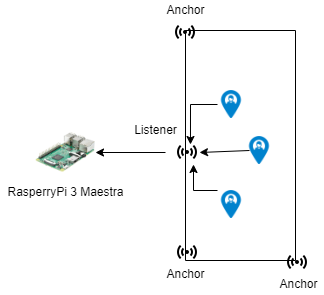
\includegraphics[width=10cm,height=10cm,keepaspectratio]{img/Esquema de coenxiones.png}
    \caption{Caso de prueba de 3 \textit{Tags}, 3 \textit{Anchors} y 1 \textit{Listener} en una sala.}
    \label{fig:app-local-representation}
\end{figure}
Los resultados fueron bastante satisfactorios llegando a una precisión de 20 cm, lo cual supera el objetivo de investigación de 50 cm de precisión en la horizontal. Al no tener diferentes plantas, finalmente no se tuvo en cuenta la precisión vertical.

También se realizó una prueba de estrés, con un script en \textit{Python}, del mapa añadiendo tags simulados a la base de datos, generando una longitud y latitud aleatorias en un rango determinado, para poder ver la frecuencia de actualización en el mapa y cuánto era límite máximo de frecuencia que permitía el mapa. En este caso los resultados fueron muy satisfactorios ya que el objetivo era trabajar insertando 1 \textit{tag} por segundo, y los resultados llegaron a 3 \textit{tags} por segundo, teniendo margen suficiente para interactuar con otras partes del sistema.
\capitulo{6}{Trabajos relacionados}
A nivel de proyecto hemos encontrado pocas ideas que a nivel global puedan formar un asistente de visitas de museos, sin embargo se puede hacer una comparación con distintos proyectos que tienen cosas en común.

Para ello compararemos los tres proyectos de investigación que se enumeran a continuación de manera separada con las distintas prestaciones que tiene nuestra aplicación:
\begin{itemize}
    \item Este proyecto \textit{open source} simula los planos de un museo permitiendo distintas interacciones del usuario con el mapa: \url{https://github.com/arcataroger/openlayers_indoor_map}
    \item La localización \textit{indoor} mediante \textit{Wifi} suele basarse en la recolección de \textit{fingerprints} de dispositivos de los usuarios, entrenar un modelo de algún algoritmo como \textit{KNN} y que prediga las ubicaciones exactas de los usuarios, este método es vulnerable al ruido en la recoleccion de datos y suele ser preciso en cuestión de metros.\cite{wifiIndoor}
    \item La localización \textit{indoor} con \textit{Bluetooth Low Energy (BLE)} se basa en medir la potencia de señal que reciben los \textit{beacons}, dispositivos que implementan \textit{BLE}, para localizarlos. Son más vulnerables que \textit{UWB} a ruido en las señales y en base a la potencia que reciba de la señal será más o menos preciso.
\end{itemize}

Se añade una tabla resumen de las métricas teóricas de cada una de las tecnologías\cite{comparacionIndoor}:
\FloatBarrier
\tablaSmall{Tabla resumen de comparación entre tecnologías para \textit{indoor positioning}.}{l c c c c}{resume-of-tec-for-positioning}{ \multicolumn{1}{l}{Tecnología} & Precisión & Rango \\}{ 
Wifi & < 15 m & < 150 m & &\\
BLE 4 & < 8 m & < 75 m & &\\
BLE 5.1 & < 1 m & < 75 m & &\\
UWB & < 30 cm & < 150 m & &\\
}{t}
\FloatBarrier

\section{Field Museum Map}

En este proyecto podemos encontrar una implementación de un mapa con la herramienta \textit{OpenLayers}, también usada en el proyecto práctico de este TFG, y desarrollado con \textit{Angular} para una \textit{webapp}, en la cual se crean diferentes salas y se insertan distintas imágenes temáticas y figuras indicadoras de dirección, que permiten a un usuario tener una experiencia más avanzada que en una visita a un museo normal. También es interesante comentar que implementa un sistema de cambio de planta, que permite dar más dinamismo a la web que está utilizando el usuario.

Sin embargo no implementa ningún tipo de geolocalización de usuarios, ni tampoco tiene ningún tipo de interacción directa de movimiento con las capas que utiliza, pero asienta las bases para poder implementarla sobre el mapa.
\FloatBarrier

\begin{figure}
    \centering
    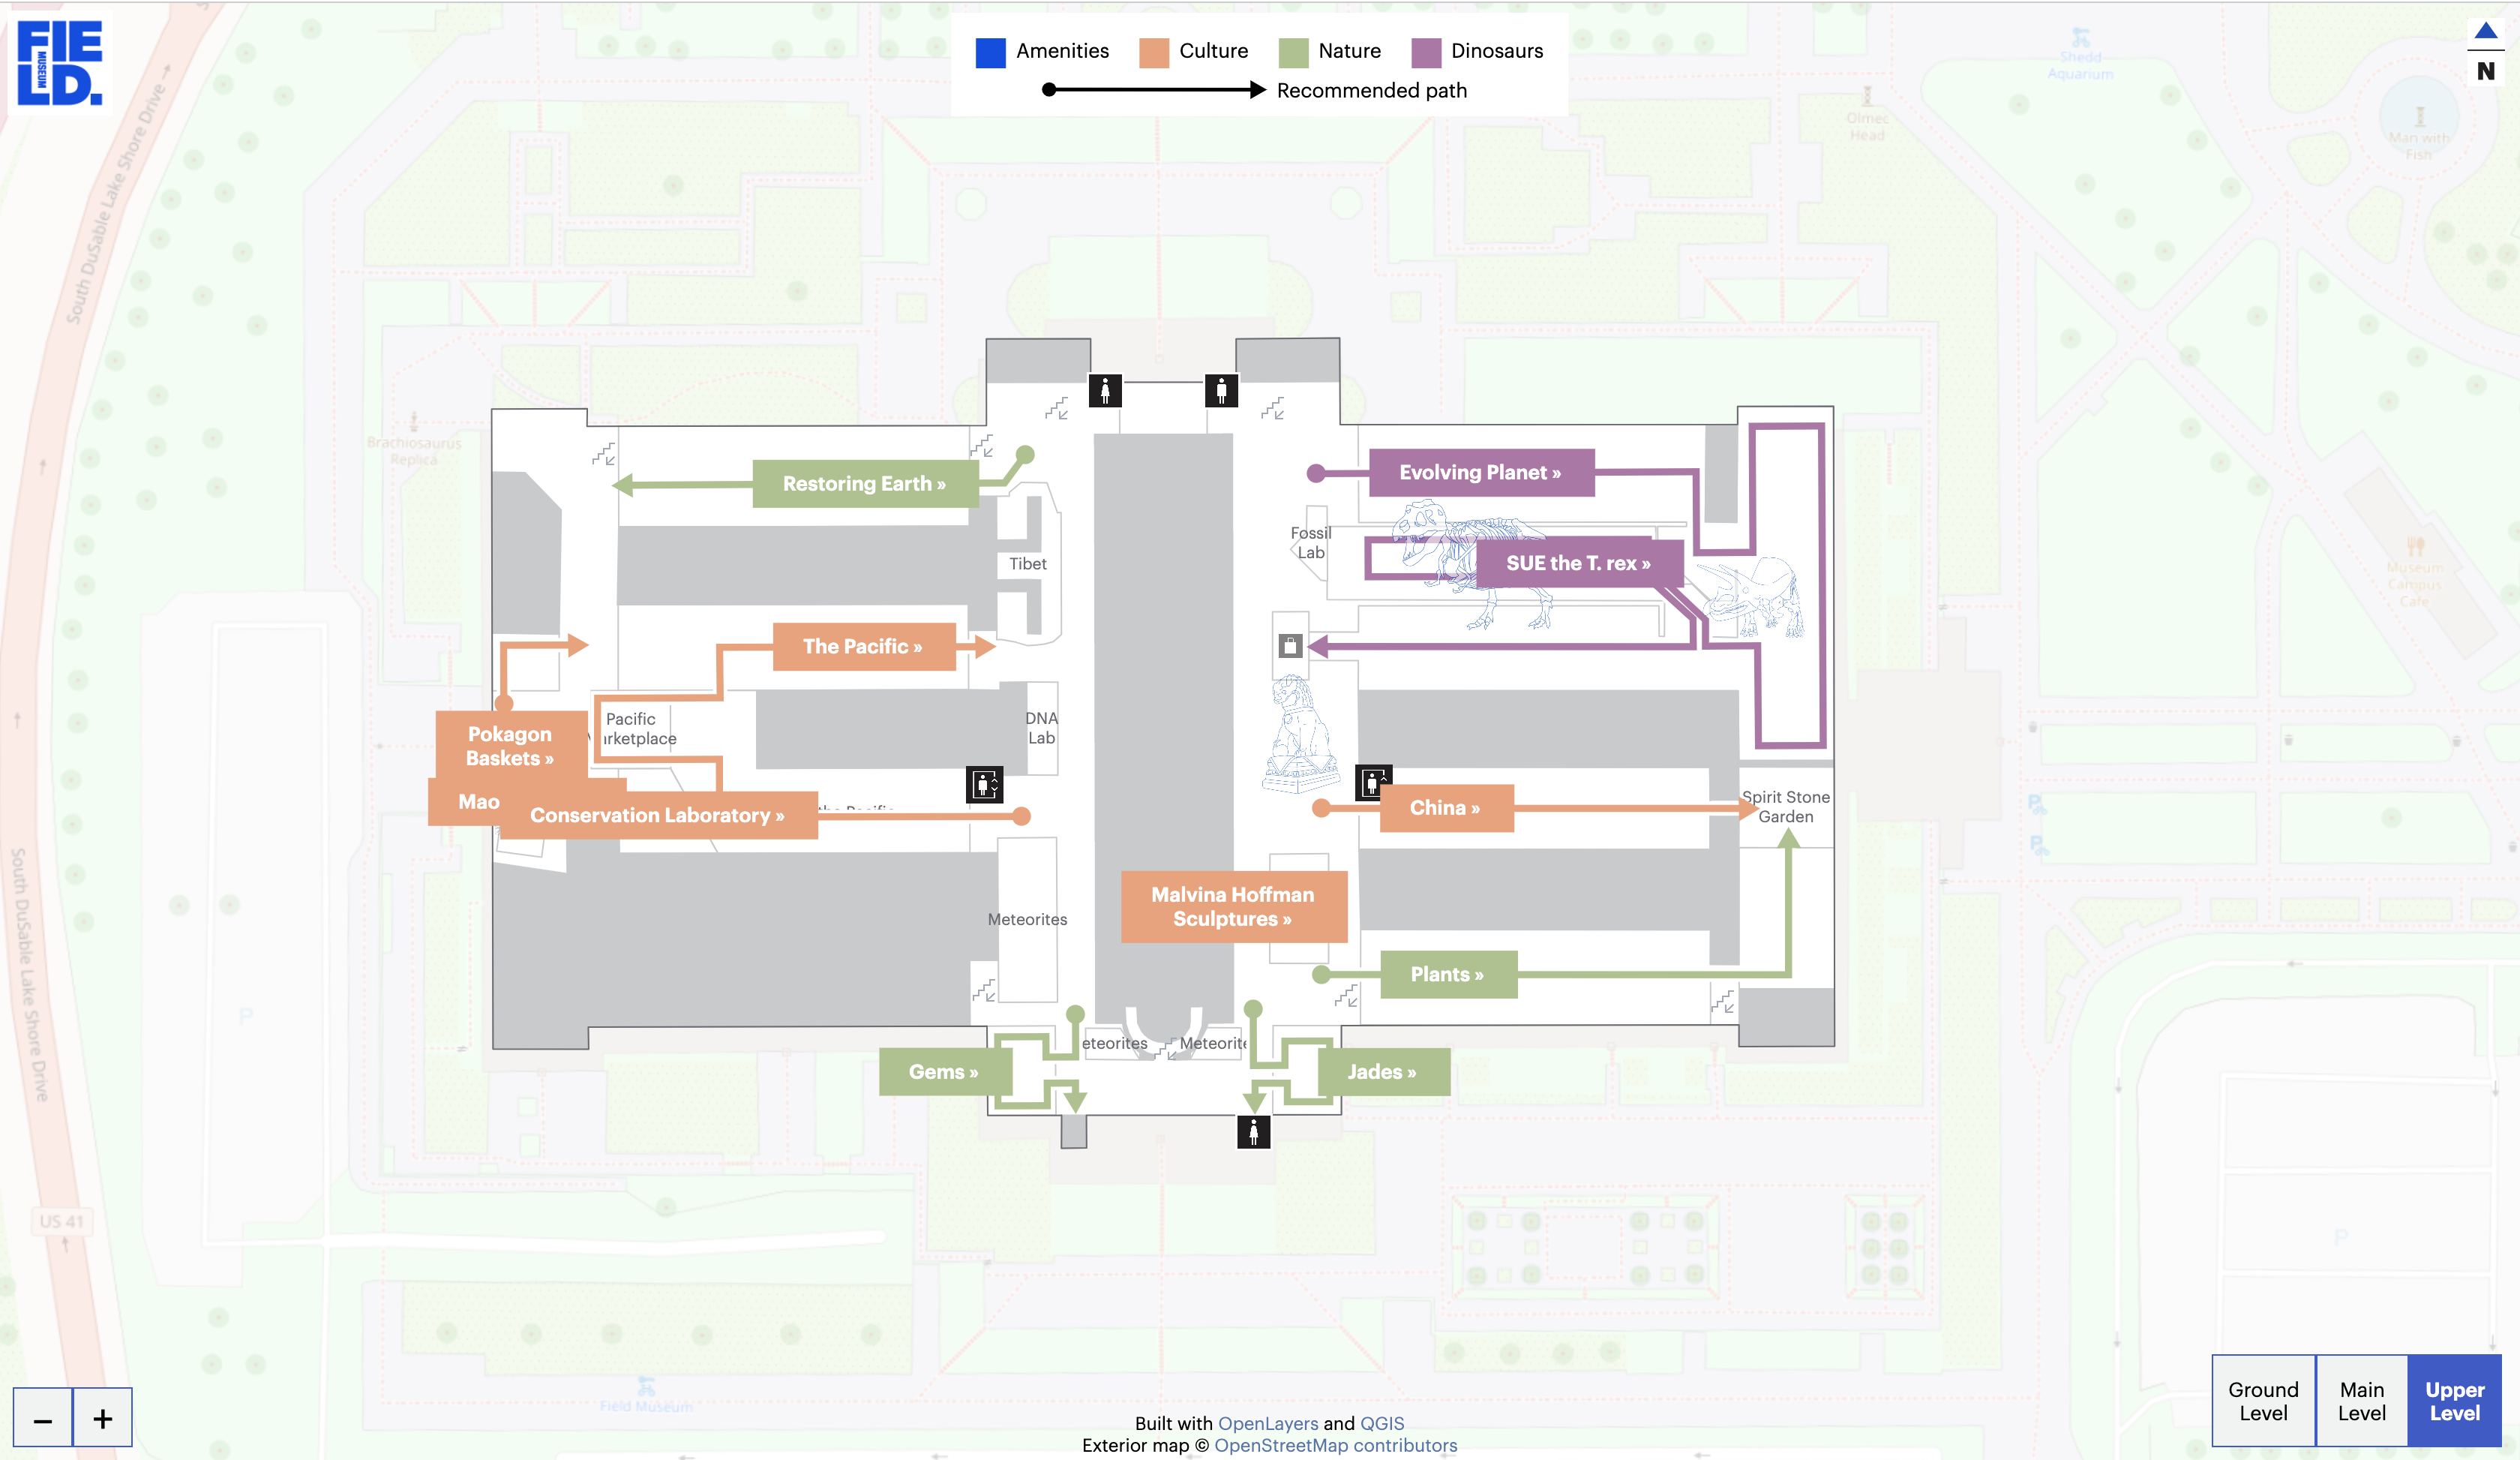
\includegraphics[width=10cm,height=10cm,keepaspectratio]{img/field_map_museum.png}
    \caption{Imagen de la Demo del proyecto \textit{Field Museum Map}.}
    \label{fig:field_museum_demo_img}
\end{figure}
\FloatBarrier

Link del proyecto: \url{https://github.com/arcataroger/openlayers_indoor_map}

Link de la Demo: \url{https://map.fieldmuseum.org/?utm_campaign=open_source&utm_source=github_readme&utm_medium=web}
\capitulo{7}{Conclusiones y Líneas de trabajo futuras}

\section{Conclusiones}
Con este proyecto se han aprendido multitud de conceptos nuevos y se han afianzado otros.

Tras la realización del proyecto se han llegado a las siguientes conclusiones:
\begin{itemize}
    \item Se ha cumplido el objetivo general del proyecto, pudiendo desarrollar un asistente para las visitas a museos enriqueciendo los tours con realidad aumentada. Para el museo se ha creado una plataforma para realizar tours de manera cómoda y pudiendo obtener información de la localización de los usuario.
    \item Se ha cumplido con el objetivo general de crear el proyecto en \textit{Open Source}.
    \item Se ha cumplido el objetivo de investigación del proyecto, pudiendo obtener una localización de los usuarios precisa, triangulada con un margen de error de aproximadamente 20 centímetros en el mapa.
    \item Se ha creado una \textit{API} para gestionar todo el flujo de datos entre la aplicación web, la base de datos y las \textit{raspberries}.
    \item Se han utilizado diversas tecnologías para la realización del proyecto. Desde \textit{React} para el desarrollo web, \textit{SQLAlchemy} y \textit{Flask} para la lógica de la \textit{API}, el uso de un archivo \textit{YAML} para el diseño de la \textit{API} y \textit{P5} para el uso de \textit{canvas} en el dibujo sobre los cuadros para la interacción con los usuarios.
\end{itemize}

\section{Líneas de trabajo futuras}
Los sistemas de posicionamiento \textit{indoor} en un museo permiten que el guía pueda gestionar flujos de gente, bien porque el guía lleve a los visitantes por sitios con poca afluencia de personas, o bien porque existan sistemas inteligentes que ayuden al visitante o al guía a diseñar una ruta de masificación de visitantes, pudiendo evitar así grandes aglomeraciones si fuese necesario, dando al usuario una mejor experiencia en la visita.

Durante el desarrollo del proyecto se han tenido en cuenta ideas que se han tenido que descartar por el límite temporal, dando margen para el desarrollo del proyecto en distintos ámbitos.

\begin{itemize}
    \item En el mapa, con el uso de un dispositivo móvil, se podría implementar el uso del giroscopio para poder dar al usuario una mejor experiencia de usuario pudiendo ver en que dirección en el mapa está, y así poderle mostrar información si esta de cara a una obra de arte mediante realidad aumentada.
    \item Se podría realizar el desarrollo de una aplicación móvil nativa para mejorar la experiencia de usuario en móviles para la realización de visitas.
    \item Se podría utilizar algún modelo entrenado para mejorar aún más la precisión de los usuario si se necesitase.
    \item Se podría emplear algún mecanismo para predecir si el usuario se va a acercar a una obra de arte. Esto combinado con el uso del giroscopio podría mejorar de manera notable la experiencia de uso en los usuarios.
    \item Se podría implementar un sistema para cambiar de planta en el mapa para el guía, cambiando así las capas que se utilizan para el render del mapa, cambiando la arquitectura de la planta y la distribución de los distintos usuarios.
    
    \item Se podría intentar mejorar la exportación de los planos del edificio al mapa sin tener que utilizar herramientas como \textit{Autocad}. Automatizando la creación de los planos de las plantas mediante algún tipo de escaneado de suelo.
    \item Se podría implementar un sistema de plantas en el mapa para museos grandes. Esto sería un característica esencial si queremos escalar la aplicación a museos grandes, ya que el guía, en un escenario realista, necesitaría cambiar de planta en muchas ocasiones para dar los tours.
    \item Se podría intentar escalar el sistema a museos con gran número de usuarios. En las pruebas se probaron hasta 200 usuarios ficticios, pero no se probaron este número de usuarios reales, ni con gran número de habitaciones, ni con distintas plantas, porque no se disponía de esta característica.
    
    \item Como última línea de trabajo se podría implementar un entorno de realidad aumentada para las \textit{HoloLens 2}. Esta línea de trabajo era inicialmente un objetivo del proyecto pero por limitaciones de tiempo no se pudo cumplir.

\end{itemize}


\bibliographystyle{plain}
\bibliography{bibliografia}

\end{document}
